\documentclass[12pt,a4paper]{book}
\usepackage[left=2cm, right=2cm, top=2.5cm, bottom=2.5cm]{geometry}
\usepackage{times}
\usepackage{natbib}
\usepackage{subfig}
\usepackage{amsmath}
\usepackage{listings}
\usepackage{longtable}
\usepackage{array}
\usepackage{booktabs}
\usepackage{caption}
\usepackage{graphicx}
\graphicspath{ {media/} }
\setlength{\parindent}{0pt}
\setlength{\parskip}{0.25cm}
\title{Fast Off-Board Charger for Electric Vehicles}

\begin{document}
\maketitle
\setcounter{tocdepth}{3}
\tableofcontents
\listoffigures
\listoftables

%%%%%%%%%%%%%%%%%%%%%%%%%%%%%%%%%%%%%%%%%%%%%%%%%%%%%%%%%%%%%%%%%%%%%%%%%%%%%%%%%%%%%%%%%%%%
\part{AC/DC Conversion}

%%%%%%%%%%%%%%%%%%%%%%%%%%%%%%%%%%%%%%%%%%%%%%%%%%%%%%%%%%%%%%%%%%%%%%%%%%%%%%%%%%%%%%%%%%%%
\chapter{Introduction to AC/DC Conversion}
The electrical power supplied by wall outlets varies globally, offering either 50Hz or 60Hz AC (Alternating Current) with a nominal voltage of approximately 120VAC or 230VAC. However, for devices like phones and laptops, which run on low voltage DC (Direct Current), an adapter is typically required. Despite the ubiquity of DC-powered electronic equipment, mains power distribution employs AC. Understanding the historical and technical reasons behind this choice provides insight into the development of our modern power systems.

AC gained prominence in distributed networks for several compelling reasons. Firstly, the early AC generators were simpler, leading to rapid improvements in reliability. Secondly, the ability to easily change the voltage using transformers became a pivotal advantage. Lastly, the use of multiple pole alternators reduced the rotation speed of more powerful generators. This three-pronged approach made AC a practical choice for widespread power distribution.

One historical obstacle for DC power distribution was introduced by Thomas Edison, who championed DC systems. Edison faced challenges as he attempted to compete with AC by using generator sets. While low voltage DC motors for step-up purposes were easy to manufacture, high-voltage DC motors for the corresponding step-down process proved unreliable, leading to frequent system breakdowns. In the end, even Edison abandoned the DC distribution concept in favor of alternating current power distribution\cite{acdc2018}.

The choice of AC over DC also considered the issue of power losses in transmission lines. As more houses were connected to the power grid, the losses in a cable with resistance (I²R loss) increased. By doubling the voltage, the current could be halved, allowing the same power cable to carry the current four times further. This principle applied to both DC and AC power transmission, but the use of transformers made it more convenient to step up the AC supply voltage for long-distance transmission and step it back down at the destination.

Currently, modern technologies enable efficient bidirectional conversion between AC and DC with high power and efficiency. While AC mains voltages are likely to remain standard soon, there is a growing interest in reconsidering DC power distribution due to our increasing dependence on electrical power. Modern power distribution involves multiple interconnected sources forming a power grid. Transmitting power over long distances (>500km) using high voltage DC has become more appealing because it eliminates impedance losses, and generators do not need to be synchronized to the same frequency or voltage.

For instance, a notable example of high voltage DC power transmission is a 2000MW link connecting England and France. This interconnection allows the two countries to exchange power based on domestic demand, highlighting the advantages of high voltage DC in a modern power grid. As technology continues to evolve, the debate between AC and DC power distribution will persist, driven by factors such as efficiency, cost, and the demands of our increasingly interconnected and power-dependent world.
%%%%%%%%%%%%%%%%%%%%%%%%%%%%%%%%%%%%%%%%%%%%%%%%%%%%%%%%%%%%%%%%%%%%%%%%%%%%%%%%%%%%%%%%%%%%

%%%%%%%%%%%%%%%%%%%%%%%%%%%%%%%%%%%%%%%%%%%%%%%%%%%%%%%%%%%%%%%%%%%%%%%%%%%%%%%%%%%%%%%%%%%%
\chapter{What is Rectification?}
Rectification refers to the process of transforming an alternating current (AC) waveform into a direct current (DC) waveform, producing a signal with a single polarity. It is essential to note that a DC voltage or current does not necessarily have to be constant; it simply means the signal's polarity remains unchanged. In some cases, a varying amplitude DC signal is referred to as pulsating DC.

The concept of rectification is fundamental in modern electronic circuits as many electronic devices require a stable, unvarying DC voltage to power their internal circuitry. Given that residential and commercial power distribution is typically in the form of AC, some form of AC to DC conversion is necessary.

Rectifiers, which perform the conversion of AC to DC, are classified into two categories based on the type of conversion: half-wave rectifiers and full-wave rectifiers. The former involves converting half cycles of AC into DC, while the latter processes full cycles of AC into DC. Understanding the differences between half-wave and full-wave rectifiers, as well as a brief exploration of each type, facilitates a clearer grasp of their distinct functionalities.
%%%%%%%%%%%%%%%%%%%%%%%%%%%%%%%%%%%%%%%%%%%%%%%%%%%%%%%%%%%%%%%%%%%%%%%%%%%%%%%%%%%%%%%%%%%%

%%%%%%%%%%%%%%%%%%%%%%%%%%%%%%%%%%%%%%%%%%%%%%%%%%%%%%%%%%%%%%%%%%%%%%%%%%%%%%%%%%%%%%%%%%%%
\section{Half-Wave Rectification}
A half-wave rectifier is a circuit that transforms only half of the alternating current (AC) cycle into direct current (DC). The typical configuration of a half-wave rectifier involves a semiconductor diode, and the circuit and output waveform are depicted in Figure \ref{fig:image1}.

\begin{figure}[h]
  \centering
  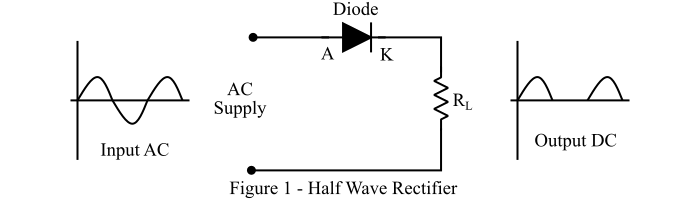
\includegraphics[width=13cm]{image1.png}
  \caption{Half-Wave Rectification Process}
  \label{fig:image1}
\end{figure}

In the process of half-wave rectification, the AC is initially stepped up or down to the desired voltage using a transformer. The transformed AC is then supplied to the diode. Here is how the rectification unfolds: During the positive half cycle of AC, the diode, operating in a forward-biased state, acts as a short circuit, allowing electric current to pass through. Conversely, during the negative half cycle of AC, the diode becomes reverse-biased, acting as an open circuit and preventing conduction. Consequently, the voltage at the load terminals is present only during the positive half cycle of AC. Thus, the alternating current is converted into direct current, flowing in a single direction, but only during one half cycle of AC.
%%%%%%%%%%%%%%%%%%%%%%%%%%%%%%%%%%%%%%%%%%%%%%%%%%%%%%%%%%%%%%%%%%%%%%%%%%%%%%%%%%%%%%%%%%%%

%%%%%%%%%%%%%%%%%%%%%%%%%%%%%%%%%%%%%%%%%%%%%%%%%%%%%%%%%%%%%%%%%%%%%%%%%%%%%%%%%%%%%%%%%%%%
\section{Full-Wave Rectification}
In contrast to half-wave rectifier, a full-wave rectifier transforms the entire cycle of alternating current into direct current. The circuit for a full-wave rectifier comprises a center-tapped step-down transformer and two semiconductor diodes. The anode terminals of the diodes connect to the secondary winding terminals of the transformer, while the cathode terminals link to a common point. The load resistor is connected between the common terminal and the center-tapping point of the transformer.

\begin{figure}[h]
  \centering
  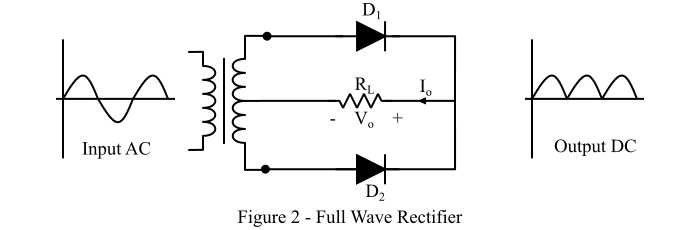
\includegraphics[width=13cm]{image2.png}
  \caption{Full-Wave Rectification Process}
  \label{fig:image2}
\end{figure}

During the positive half cycle of AC, diode D\textsubscript{1} is forward biased, and diode D\textsubscript{2} is reverse biased. Consequently, diode D\textsubscript{1} conducts, allowing current to flow through D\textsubscript{1} and the load resistor R\textsubscript{L}. In the negative half cycle of AC, the situation reverses: diode D\textsubscript{1} becomes reverse biased, and diode D\textsubscript{2} becomes forward biased. Only diode D\textsubscript{2} is conducted during this negative half cycle, and the current flows through D\textsubscript{2} and the load resistor R\textsubscript{L}. The circuit and output voltage waveform for the full-wave rectifier are illustrated in Figure \ref{fig:image2}. This way, a full-wave rectifier efficiently converts the entire AC cycle into DC \cite{rectifier2023}.

While the explanations above focus on a single-phase AC system, they can be extended to three-phase systems commonly used in fast-charging offboard chargers. In a three-phase half-wave rectifier, the system requires three diodes, and for the full-bridge system, six diodes are necessary. The adaptability of rectification principles to different configurations underscores their significance in converting AC to DC, a crucial requirement for many electronic devices and power systems.
%%%%%%%%%%%%%%%%%%%%%%%%%%%%%%%%%%%%%%%%%%%%%%%%%%%%%%%%%%%%%%%%%%%%%%%%%%%%%%%%%%%%%%%%%%%%

%%%%%%%%%%%%%%%%%%%%%%%%%%%%%%%%%%%%%%%%%%%%%%%%%%%%%%%%%%%%%%%%%%%%%%%%%%%%%%%%%%%%%%%%%%%%
\chapter{Topologies for AC/DC Conversion Stage}
The AC-DC converter of an offboard charger is a front-end rectifier before the DC-DC conversion stage of the complete EV fast charging station. Various topologies are available that convert AC power from the utility grid to DC power. Such topologies are expected to manage high power fed directly to the battery as part of an EV fast charging solution. 
%%%%%%%%%%%%%%%%%%%%%%%%%%%%%%%%%%%%%%%%%%%%%%%%%%%%%%%%%%%%%%%%%%%%%%%%%%%%%%%%%%%%%%%%%%%%

%%%%%%%%%%%%%%%%%%%%%%%%%%%%%%%%%%%%%%%%%%%%%%%%%%%%%%%%%%%%%%%%%%%%%%%%%%%%%%%%%%%%%%%%%%%%
\section{Three-Phase Passive Rectifier}
The simplest rectifier configuration is the three-phase diode rectifier, comprising six diodes, AC side inductors, and a DC side capacitor (refer to \ref{fig:image3}).

\begin{figure}[h]
  \centering
  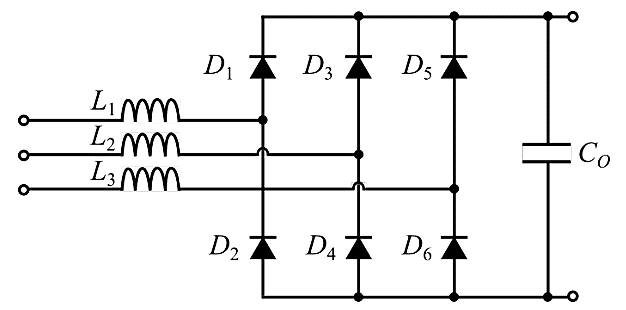
\includegraphics[width=10cm]{image3.png}
  \caption{Three-Phase Passive Rectifier}
  \label{fig:image3}
\end{figure}

As it runs without active switches, this converter drops the need for a control system or gate drivers, streamlining its functionality. Diodes switch at the grid frequency without active current shaping or control over the output voltage. However, diode rectifiers can introduce a Total Harmonic Distortion (THD) of 40–70\% into grid currents, potentially stressing the grid, especially with numerous fast high-power passive rectifiers. Due to its lower efficiency, unidirectional power flow, and higher THD, this conventional passive rectifier topology is not recommended for fast charging applications.

Unlike passive rectifiers, active rectifiers, when employed, allow for controlled DC link voltage, keeping the desired voltage level across varying loads. This helps minimize THD, achieving both high efficiency and power factor. The later comparison focuses on three boost-type bidirectional active converters: Three-phase two-level six-switch boost-type rectifier, Three-phase three-level neutral point clamped converter, and Three-phase three-level T-type converter.
%%%%%%%%%%%%%%%%%%%%%%%%%%%%%%%%%%%%%%%%%%%%%%%%%%%%%%%%%%%%%%%%%%%%%%%%%%%%%%%%%%%%%%%%%%%%

%%%%%%%%%%%%%%%%%%%%%%%%%%%%%%%%%%%%%%%%%%%%%%%%%%%%%%%%%%%%%%%%%%%%%%%%%%%%%%%%%%%%%%%%%%%%
\section{Three-Phase Vienna Rectifier}
The three-phase Vienna rectifier, illustrated in \ref{fig:image4}, includes three input inductors for voltage boosting, followed by six diodes for rectification and six semiconductor switches. Additionally, two split capacitors are incorporated in the output. Its functioning is akin to a traditional three-phase boost Power Factor Correction (PFC) rectifier, but unlike the latter, it does not ease bidirectional power flow. The Vienna rectifier employs a straightforward control mechanism, ensuring unity power factor operation and minimizing Total Harmonic Distortion (THD). Its notable efficiency, particularly in power-dense applications, makes it well-suited for high-power scenarios such as fast-charging Electric Vehicles (EVs).

\begin{figure}[h]
  \centering
  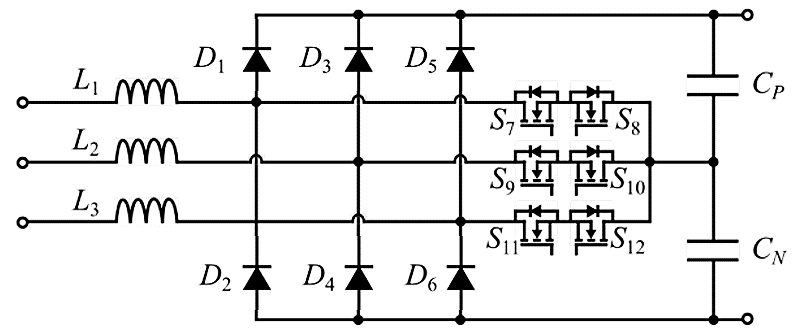
\includegraphics[width=10cm]{image4.png}
  \caption{Three-Phase Vienna Rectifier}
  \label{fig:image4}
\end{figure}

To enable bidirectional power flow, the Vienna rectifier can be changed by replacing diodes with switches, a modification especially beneficial in Vehicle-to-Grid (V2G) applications. The Vienna rectifier typically runs using modulation methods like carrier-based Pulse Width Modulation (PWM), Space Vector PWM, and discontinuous PWM. However, in the case of interleaved Vienna rectifiers, Space Vector PWM can introduce distortions in input current waveforms, while the other two PWM techniques may lead to undesirable ripples. To address these challenges, a hybrid Space Vector PWM approach is employed, effectively mitigating the issues associated with the modulation techniques.
%%%%%%%%%%%%%%%%%%%%%%%%%%%%%%%%%%%%%%%%%%%%%%%%%%%%%%%%%%%%%%%%%%%%%%%%%%%%%%%%%%%%%%%%%%%%

%%%%%%%%%%%%%%%%%%%%%%%%%%%%%%%%%%%%%%%%%%%%%%%%%%%%%%%%%%%%%%%%%%%%%%%%%%%%%%%%%%%%%%%%%%%%
\section{Three-Phase Two-Level Six-Switch Boost-Type Rectifier}
The configuration for the three-phase two-level boost-type rectifier is depicted in \ref{fig:image5}. It forms six active switches (MOSFETs or IGBTs), AC side boost inductors, and a DC side filter capacitor. Known for its simplicity, robustness, and familiarity, the two-level six-switch rectifier topology needs larger-volume input inductors and is constrained by a maximum switching frequency compared to three-level converters.

\begin{figure}[h]
  \centering
  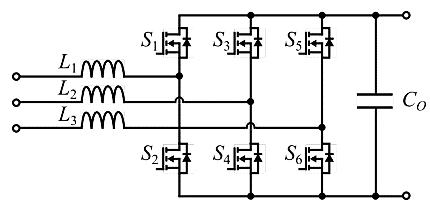
\includegraphics[width=10cm]{image5.png}
  \caption{Three-Phase Two-Level Six-Switch Boost-Type Rectifier}
  \label{fig:image5}
\end{figure}

The rectifier, being of a boosting nature, imposes a lower limit on the DC link voltage. For instance, if the rectifier is connected to a three-phase grid with a 400 V RMS line-to-line voltage, the smallest DC link voltage would be 565 V, equal to the line-to-line voltage amplitude. Ideally, keeping a DC link voltage 15–20% higher is recommended to mitigate distortion in current waveforms.

In a two-level topology line-to-neutral rectifier, the voltage is either zero or matches the DC link voltage. Consequently, this gives rise to a three-level line-to-line voltage.
%%%%%%%%%%%%%%%%%%%%%%%%%%%%%%%%%%%%%%%%%%%%%%%%%%%%%%%%%%%%%%%%%%%%%%%%%%%%%%%%%%%%%%%%%%%%

%%%%%%%%%%%%%%%%%%%%%%%%%%%%%%%%%%%%%%%%%%%%%%%%%%%%%%%%%%%%%%%%%%%%%%%%%%%%%%%%%%%%%%%%%%%%
\section{Three-Phase Three-Level Neutral Point Clamped Converter }
The configuration of a three-phase three-level neutral point clamped (NPC) converter is illustrated in \ref{fig:image6}. Comprising twelve active switches, six diodes, and filters, this three-level topology offers advantages over the two-level converter. Notably, switches in this arrangement experience reduced voltage stress and lower switching losses, while the passive filter size is also smaller. However, the trade-off involves an increased part count, leading to potential drawbacks in system reliability, complexity, and implementation effort.

\begin{figure}[h]
  \centering
  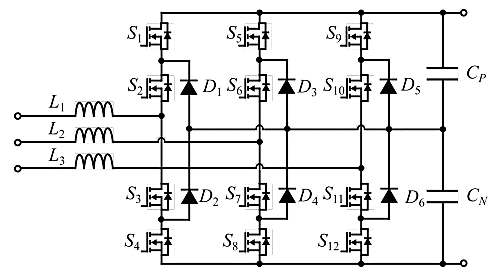
\includegraphics[width=10cm]{image6.png}
  \caption{Three-Phase Three-Level Neutral Point Clamped Converter}
  \label{fig:image6}
\end{figure}

In a three-level topology, the line-to-neutral voltage can take values of 0.5 VDC, zero, or -0.5 VDC, resulting in a five-level line-to-line voltage. Despite the increase in complexity, the NPC converter keeps a sinusoidal grid side current similar to the two-level topology, featuring harmonics around the switching frequency and its multiples during harmonic analysis.

The primary limitation of the NPC topology lies in its use of twelve active and six passive switches, resulting in increased costs and complexity. Despite these drawbacks, it offers notable advantages such as a substantial reduction in inductor size and ensures that all switches are exposed to only half the DC link voltage. However, this configuration needs two capacitors in series, leading to higher capacitance values and lower capacitor voltage ratings.
%%%%%%%%%%%%%%%%%%%%%%%%%%%%%%%%%%%%%%%%%%%%%%%%%%%%%%%%%%%%%%%%%%%%%%%%%%%%%%%%%%%%%%%%%%%%

%%%%%%%%%%%%%%%%%%%%%%%%%%%%%%%%%%%%%%%%%%%%%%%%%%%%%%%%%%%%%%%%%%%%%%%%%%%%%%%%%%%%%%%%%%%%
\section{Three-Phase Three-Level T-Type Converter}
Three-phase three-level T-type converter is a bidirectional variation of the three-phase Vienna rectifier. The topology is shown in \ref{fig:image7}. This rectifier uses twelve active switches, compared to the original unidirectional topology that uses six diodes and six active switches. Moreover, it has three boost inductors on the AC side and a split capacitor on the DC side. This is a three-level topology similar to NPC. However, it has lower semiconductor losses for low switching frequencies compared to NPC, and it can be implemented using standard six-pack modules. This topology uses switches for two different voltage ratings.
\begin{figure}[h]
  \centering
  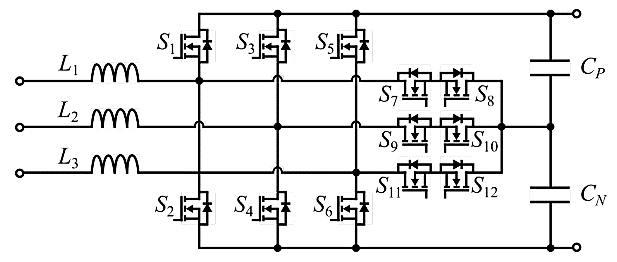
\includegraphics[width=10cm]{image7.png}
  \caption{Three-Phase Three-Level T-Type Converter}
  \label{fig:image7}
\end{figure}

The three-level T-type rectifier also generates a three-level line-to-neutral voltage and five-level line-to-line voltage. The current is quite similar to the NPC converter current, also it uses similar filter sizes and filter ratings as the NPC. The main difference is the number and rating of the switches. 

The two switches between positive and negative DC link block voltages between 0.5 VDC and VDC, so they must be rated for VDC. However, when these devices are switching, the voltage level changes between zero and 0.5 VDC, which results in lower switching losses compared to switching with full VDC. The devices connected between the phase leg midpoint and DC link midpoint block 0.5 VDC, so they only need to be rated for 0.5 VDC. Moreover, they also switch between zero and 0.5 VDC. Overall, the reduced number of components compared to NPC, while keeping switching from 0.5 VDC, results in higher efficiency than NPC. The efficiency of the T-type rectifier at full load is 98.95\%.
%%%%%%%%%%%%%%%%%%%%%%%%%%%%%%%%%%%%%%%%%%%%%%%%%%%%%%%%%%%%%%%%%%%%%%%%%%%%%%%%%%%%%%%%%%%%

%%%%%%%%%%%%%%%%%%%%%%%%%%%%%%%%%%%%%%%%%%%%%%%%%%%%%%%%%%%%%%%%%%%%%%%%%%%%%%%%%%%%%%%%%%%%
\chapter{Implementation of Closed-Loop AC/DC Converter}
We will now address challenges through the design and implementation of a closed-loop AC/DC rectifier system. The closed-loop architecture, with its feedback mechanism, promises not only enhanced control over the rectification process but also the mitigation of issues associated with traditional rectifiers. The journey towards an optimized closed-loop system involves a meticulous exploration of key components, each playing a pivotal role in achieving the desired efficiency and stability.

The aims of this research encompass a detailed examination of critical aspects, including filter selection, DC-link configuration, phase-locked loop (PLL), Clarke and Park transformations, and Proportional-Integral-Derivative (PID) control. 
%%%%%%%%%%%%%%%%%%%%%%%%%%%%%%%%%%%%%%%%%%%%%%%%%%%%%%%%%%%%%%%%%%%%%%%%%%%%%%%%%%%%%%%%%%%%

%%%%%%%%%%%%%%%%%%%%%%%%%%%%%%%%%%%%%%%%%%%%%%%%%%%%%%%%%%%%%%%%%%%%%%%%%%%%%%%%%%%%%%%%%%%%
\section{Proportional Integral Derivative (PID)}
A proportional–integral–derivative controller (PID controller) is a control loop mechanism employing feedback that is widely used in industrial control systems and a variety of other applications requiring continuously modulated control. As implied by its name, the PID controller combines proportional control with added integral and derivative adjustments, helping the unit to automatically compensate for changes in a system. 

Proportional-Integral-Derivative (PID) control is the most common control algorithm used in industry and has been universally accepted in industrial control. The popularity of PID controllers can be attributed partly to their robust performance in a wide range of operating conditions and partly to their functional simplicity, which allows engineers to run them in a simple, straightforward manner. The PID algorithm consists of three basic coefficients; proportional, integral, and derivative which are varied to get best response. 

PID controller keeps the output such that there is zero error between process variable and set point (desired output) by closed loop operations and tuning PID parameters. PID uses three basic control behaviors. 
%%%%%%%%%%%%%%%%%%%%%%%%%%%%%%%%%%%%%%%%%%%%%%%%%%%%%%%%%%%%%%%%%%%%%%%%%%%%%%%%%%%%%%%%%%%%
\subsection{P-Controller}
Proportional or P- controller gives an output that is proportional to error e(t). It compares the desired or set point with the actual value or feedback process value. 

\begin{figure}[h]
  \centering
  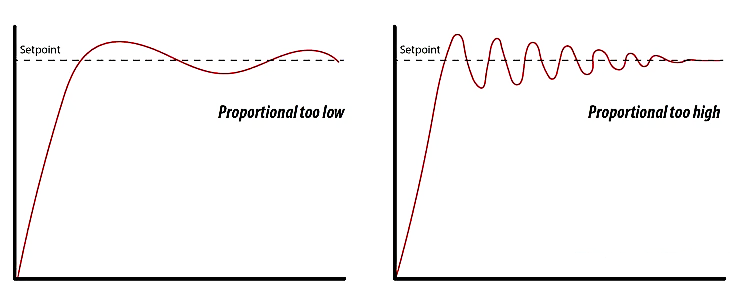
\includegraphics[width=15cm]{image8.png}
  \caption{The Effect of P-Gain on a System}
  \label{fig:image8}
\end{figure}

The resulting error is multiplied with a proportional constant to get the output. If the error value is zero, then this controller output is zero. This controller requires biasing or manual reset when used alone. This is because it never reaches the steady-state condition. It supplies stable operation but always keeps the steady-state error. The speed of the response is increased when the proportional constant KP increases. P-Controller Equation:
\begin{equation}
  u\left(t\right)=K_pe(t)
  \label{equation:eq1}
\end{equation}

%%%%%%%%%%%%%%%%%%%%%%%%%%%%%%%%%%%%%%%%%%%%%%%%%%%%%%%%%%%%%%%%%%%%%%%%%%%%%%%%%%%%%%%%%%%%

%%%%%%%%%%%%%%%%%%%%%%%%%%%%%%%%%%%%%%%%%%%%%%%%%%%%%%%%%%%%%%%%%%%%%%%%%%%%%%%%%%%%%%%%%%%%
\subsection{I-Controller}
Due to the limitation of p-controller where there always exists an offset between the process variable and setpoint, I-controller is needed, which supplies necessary action to cut the steady-state error.

\begin{figure}[h]
  \centering
  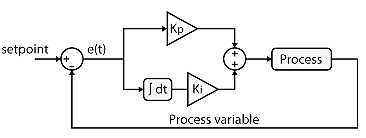
\includegraphics[width=10cm]{image9.png}
  \caption{PI-Control Process}
  \label{fig:image9}
\end{figure}

It integrates the error over a period of time until the error value reaches zero. It holds the value to the final control device at which the error becomes zero. Integral control decreases its output when a negative error takes place. It limits the speed of response and affects the stability of the system. The speed of the response is increased by decreasing integral gain, Ki. PI-Controller Equation:
\begin{equation}
  u\left(t\right)=K_pe\left(t\right)+K_i\int_{0}^{t}{e\left(\tau\right)\ d\tau}
  \label{equation:eq2}
\end{equation}
%%%%%%%%%%%%%%%%%%%%%%%%%%%%%%%%%%%%%%%%%%%%%%%%%%%%%%%%%%%%%%%%%%%%%%%%%%%%%%%%%%%%%%%%%%%%

%%%%%%%%%%%%%%%%%%%%%%%%%%%%%%%%%%%%%%%%%%%%%%%%%%%%%%%%%%%%%%%%%%%%%%%%%%%%%%%%%%%%%%%%%%%%
\subsection{D-Controller}
I-controller does not have the capability to predict the future behavior of error. So, it reacts normally once the setpoint is changed. D-controller overcomes this problem by expecting the future behavior of the error. Its output depends on the rate of change of error with respect to time, multiplied by derivative constant. It gives the kick start for the output thereby increasing system response.

\begin{figure}[h]
  \centering
  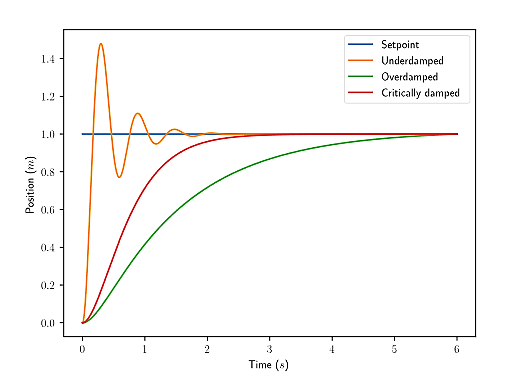
\includegraphics[width=14cm]{image10.png}
  \caption{PID Control on a System}
  \label{fig:image10}
\end{figure}

In \ref{fig:image10}, response of D, the controller is more, compared to the PI controller, and also settling time of output is decreased. It improves the stability of the system by compensating for phase lag caused by I- controller. PID Controller Equation: 
\begin{equation}
  u\left(t\right)=K_pe\left(t\right)+K_i\int_{0}^{t}{e\left(\tau\right)\ d\tau}+K_d\frac{de(t)}{dt}
  \label{equation:eq3}
\end{equation}

The following figure shows the structure of the PID controller. It consists of a PID block which gives its output to the process block. Process/plant consists of final control devices like actuators, control valves, and other control devices to control various processes of industry/plant. A feedback signal from the process plant is compared with a set point or reference signal r(t) and the corresponding error signal e(t) is fed to the PID algorithm.

\begin{figure}[h]
  \centering
  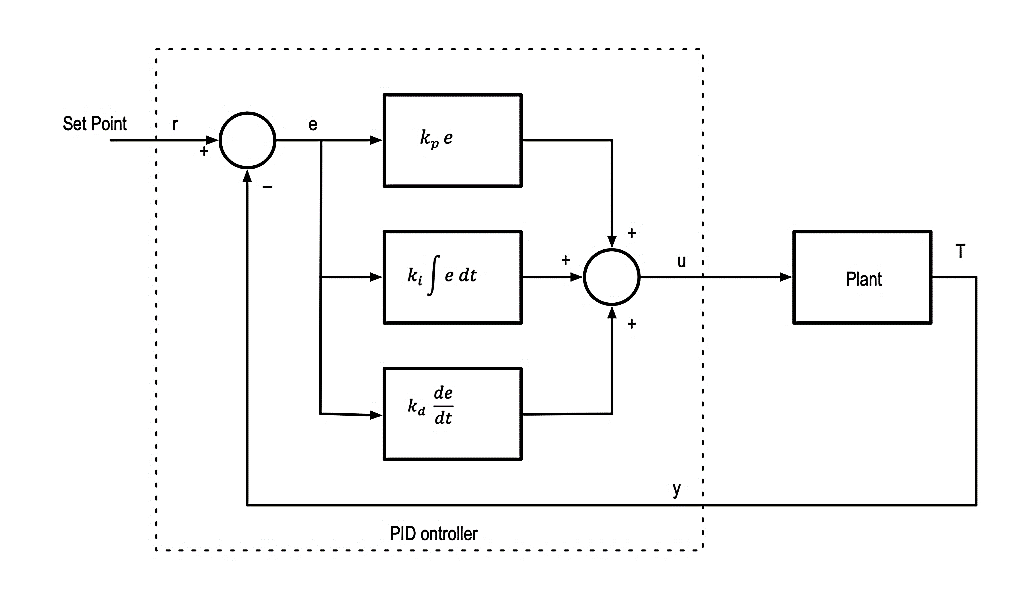
\includegraphics[width=12cm]{image11.png}
  \caption{PID Control Process}
  \label{fig:image11}
\end{figure}

According to the proportional, integral, and derivative control calculations in the algorithm, the controller produces a combined response or controlled output which is applied to plant control devices.
%%%%%%%%%%%%%%%%%%%%%%%%%%%%%%%%%%%%%%%%%%%%%%%%%%%%%%%%%%%%%%%%%%%%%%%%%%%%%%%%%%%%%%%%%%%%

%%%%%%%%%%%%%%%%%%%%%%%%%%%%%%%%%%%%%%%%%%%%%%%%%%%%%%%%%%%%%%%%%%%%%%%%%%%%%%%%%%%%%%%%%%%%
\subsection{Tuning of PID Controller}
Before the working of PID controller takes place, it must be tuned to suit the dynamics of the process to be controlled. Several types of tuning methods are developed to tune the PID controllers and require much attention to select the best values of proportional, integral, and derivative gains. Some of these methods are Trial and Error method, Process reaction curve technique and Zeigler-Nichol’s method. We used Trial and Error method in our project as it is simple and time effective. It is done by firstly setting ki to zero then increasing kp until the system reaches oscillating behavior at constant rate. Once it is oscillating, it is time to adjust ki so that oscillations are reduced.
%%%%%%%%%%%%%%%%%%%%%%%%%%%%%%%%%%%%%%%%%%%%%%%%%%%%%%%%%%%%%%%%%%%%%%%%%%%%%%%%%%%%%%%%%%%%

%%%%%%%%%%%%%%%%%%%%%%%%%%%%%%%%%%%%%%%%%%%%%%%%%%%%%%%%%%%%%%%%%%%%%%%%%%%%%%%%%%%%%%%%%%%%
\subsection{The Main Control Circuit}
The following figure shows the main control circuit which is used to control the voltage with the outer loop and the current with the inner loop and finally generates the corresponding PWM signals that are used to run and control the inverter.

\begin{figure}[h]
  \centering
  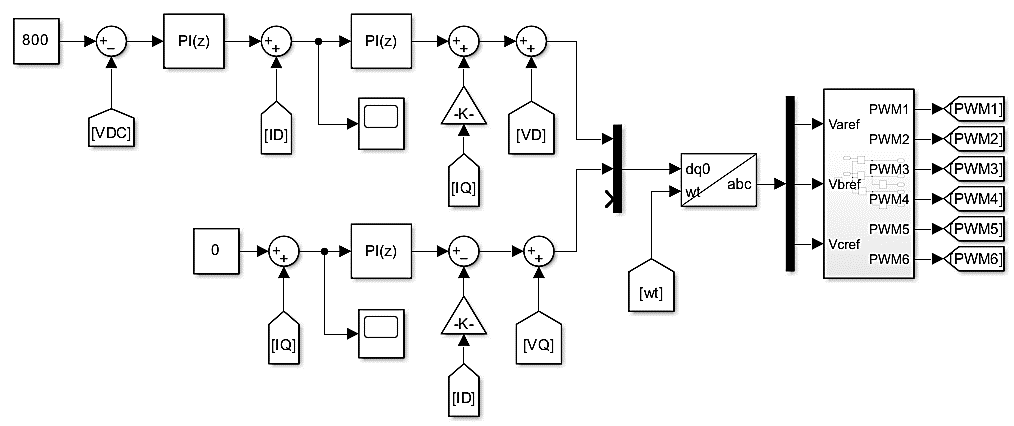
\includegraphics[width=15cm]{image12.png}
  \caption{Control Circuit of AFE with 800V Output Voltage}
  \label{fig:image12}
\end{figure}

There are a lot of methods to control but we used a Voltage Oriented Control for its simplicity \cite{pid2015}.
In voltage-oriented control (VOC), the line input current is orientedwith respect to the line voltage vector. The line voltage vector can be obtained by measurement by using sensors or estimation. In synchronous rotating reference frame, the d-axis is aligned with the line voltage vector. The d-axis component of the line current ``id'' is proportional to the active power and its q-axis component is proportional to reactive power. To achieve unity power factor the reactive component of current reference\(\ \mathbf{i}_{\mathbf{q}}^{\mathbf{*}}\) is set to zero. While the active component of current reference \(\mathbf{i}_{\mathbf{d}}^{\mathbf{*}}\mathbf{\ }\)is obtained from the PI controller, which gives the output by comparing the dc link voltage at the output with the reference voltage set as per the load requirements.

\begin{figure}[h]
  \centering
  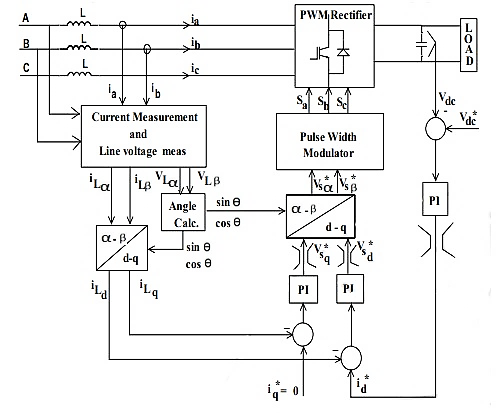
\includegraphics[width=15cm]{image13.png}
  \caption{PI Control Loop of AFE}
  \label{fig:image13}
\end{figure}

Coupling occurs due to voltage drop across inductors due to orthogonal current component coming in phase with the voltage components. Decoupling is essential to have proper control.
\begin{equation}
  V_{sd}=\ V_{ld}-L\frac{{di}_d}{dt}+\omega Li_q
  \label{equation:eq4}
\end{equation}
\begin{equation}
  V_{sq}=\ V_{lq}-L\frac{{di}_q}{dt}-\omega Li_d
  \label{equation:eq5}
\end{equation}

The voltage Vlq is zero by aligning the line voltage vector along the d-axis and q-axis current is regulated to zero.
The current controller is decoupled as
\begin{equation}
  V_{sd} = \omega Li_{lq} + \ V_{ld} + {\mathrm{\Delta}V}_{d}
  \label{equation:eq6}
\end{equation}
\begin{equation}
  V_{sq} = - \omega Li_{ld} + \mathrm{\Delta}V_{q}
  \label{equation:eq7}
\end{equation}

where
\begin{equation}
  \mathrm{\Delta}Vd = K_{p}\left( i_{d}^{*} - i_{d} \right) + K_{i}\int_{}^{}{\left( i_{d}^{*} - i_{d} \right)dt}
  \label{equation:eq8}
\end{equation}
\begin{equation}
  {\mathrm{\Delta}V}_{q} = K_{p}\left( i_{q}^{*} - i_{q} \right) + K_{i}\int_{}^{}{\left( i_{q}^{*} - i_{q} \right)dt}
  \label{equation:eq9}
\end{equation}
In VOC it is possible to calculate the voltage across the input inductor by differentiating the current flowing through it. It is then possible to estimate the line voltage by adding voltage drop across the inductor with rectifier input voltage.
%%%%%%%%%%%%%%%%%%%%%%%%%%%%%%%%%%%%%%%%%%%%%%%%%%%%%%%%%%%%%%%%%%%%%%%%%%%%%%%%%%%%%%%%%%%%

%%%%%%%%%%%%%%%%%%%%%%%%%%%%%%%%%%%%%%%%%%%%%%%%%%%%%%%%%%%%%%%%%%%%%%%%%%%%%%%%%%%%%%%%%%%%
\section{Phase-Locked Loop (PLL)}
The reason why we need PLL is: suppose we want to send an active current to the grid the current should be in phase with the voltage that means that for grid connected inverters we need synchronization, so a reference signal is generated which is in phase with the actual voltage with an amplitude of 1, -1 using phase-locked loop (PLL).

The signal is used as a reference for the implementation of current controller in the grid connected inverters. There are two methods of phase locked loop implementation:
%%%%%%%%%%%%%%%%%%%%%%%%%%%%%%%%%%%%%%%%%%%%%%%%%%%%%%%%%%%%%%%%%%%%%%%%%%%%%%%%%%%%%%%%%%%%
\subsection{Method I}
Here ABC voltages are converted into \(\alpha\), \(\beta\) voltages taking the equation shown in the diagram below giving us the angle information and from this angle information we generate reference signal but, there are few problems with this method and not used in many applications. 

\begin{figure}[h]
  \centering
  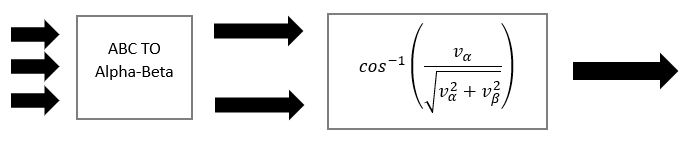
\includegraphics[width=13cm]{image0.png}
  \label{fig:image0}
\end{figure}

The problems are mainly:
\begin{itemize}
  \item It is merely an algebraic method with simple mathematics involved.
  \item Open loop system so any outer effects or conditions can lead the grid to unstable condition so PLL cannot withstand harmonics, surges, noise, and spikes.
  \item Drift of angle and giving wrong angle information due to the mentioned effects.
\end{itemize}
But we can get rid of these problems by using closed loop phase locked loop (PLL).
%%%%%%%%%%%%%%%%%%%%%%%%%%%%%%%%%%%%%%%%%%%%%%%%%%%%%%%%%%%%%%%%%%%%%%%%%%%%%%%%%%%%%%%%%%%%

%%%%%%%%%%%%%%%%%%%%%%%%%%%%%%%%%%%%%%%%%%%%%%%%%%%%%%%%%%%%%%%%%%%%%%%%%%%%%%%%%%%%%%%%%%%%
\subsection{Method II}
Here we also start by transforming ABC signals into \(\alpha - \beta\) signals then into dq voltages as shown in the figure below.

\begin{figure}[h]
  \centering
  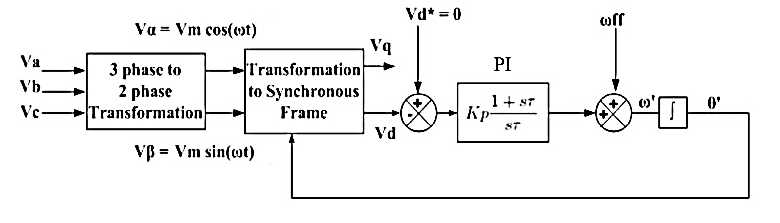
\includegraphics[width=13cm]{image14.png}
  \caption{PLL Control}
  \label{fig:image14}
\end{figure}

We can observe from the phasor diagram that D-axis is not aligned with the grid voltage so, by using the control mechanism shown in the figure we can make Vq = 0 using a PI controller and then the o/p is given to an integrator to find \(\omega t\).

\begin{figure}[h]
  \centering

  \subfloat[With q-Component]{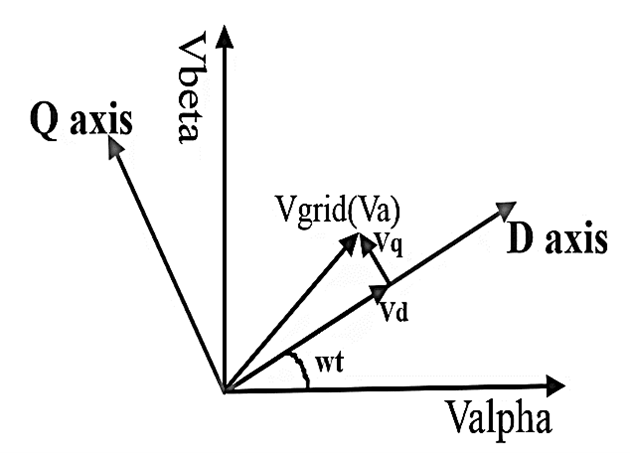
\includegraphics[width=0.5\textwidth]{image15_a.png}\label{fig:image15_a}}
  \hfill
  \subfloat[Without q-Component]{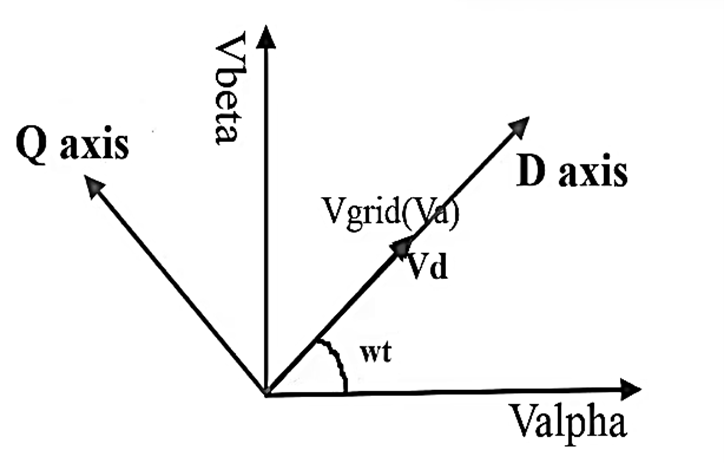
\includegraphics[width=0.5\textwidth]{image15_b.png}\label{fig:image15_b}}

  \caption{\(\alpha - \beta\) Signals to d-q Signals}
  \label{fig:image15}
\end{figure}

After making the Vq equal to zero the D-axis got aligned with the grid voltage and the angle between alpha-component and the D-axis has also changed to a new value which will the angle used in generating the reference signal.
%%%%%%%%%%%%%%%%%%%%%%%%%%%%%%%%%%%%%%%%%%%%%%%%%%%%%%%%%%%%%%%%%%%%%%%%%%%%%%%%%%%%%%%%%%%%

%%%%%%%%%%%%%%%%%%%%%%%%%%%%%%%%%%%%%%%%%%%%%%%%%%%%%%%%%%%%%%%%%%%%%%%%%%%%%%%%%%%%%%%%%%%%
\section{Clarke and Park Transformations}
Clarke and Park transforms are commonly used in field-oriented control of three-phase AC machines. The Clarke transform converts the time domain components of a three-phase system (in ABC frame) to two components in an orthogonal stationary frame (\(\alpha - \beta\)). The Park transform converts the two components in the \(\alpha - \beta\) frame to an orthogonal rotating reference frame (d-q). Implementing these two transforms in a consecutive manner simplifies computations by converting AC current and voltage waveform into DC signals.

\begin{figure}[h]
  \centering
  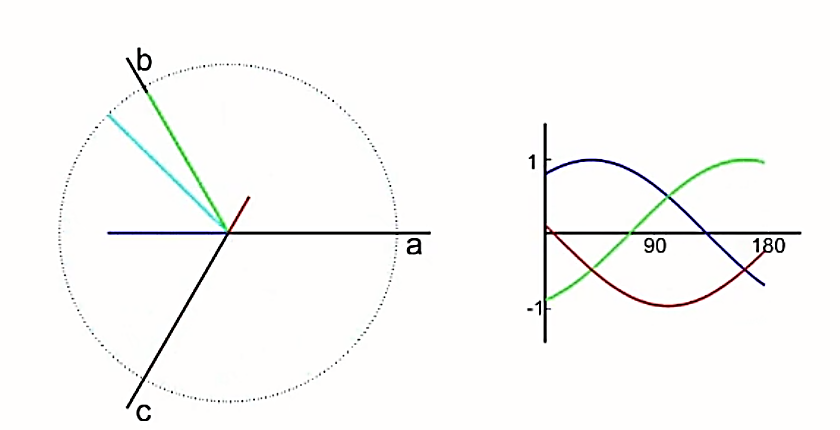
\includegraphics[width=12cm]{image16.png}
  \caption{ABC Frame}
  \label{fig:image16}
\end{figure}
%%%%%%%%%%%%%%%%%%%%%%%%%%%%%%%%%%%%%%%%%%%%%%%%%%%%%%%%%%%%%%%%%%%%%%%%%%%%%%%%%%%%%%%%%%%%

%%%%%%%%%%%%%%%%%%%%%%%%%%%%%%%%%%%%%%%%%%%%%%%%%%%%%%%%%%%%%%%%%%%%%%%%%%%%%%%%%%%%%%%%%%%%
\subsection{Clarke Transform}

\begin{figure}[h]
  \centering
  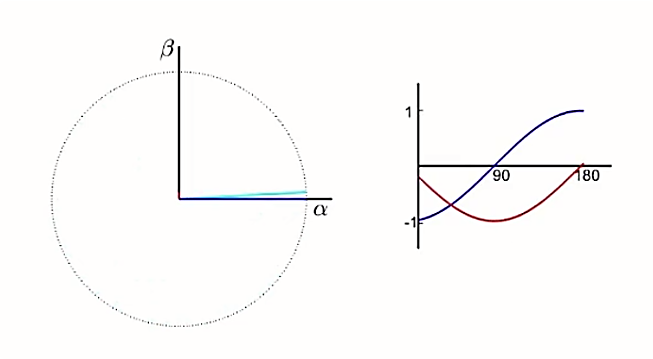
\includegraphics[width=12cm]{image17.png}
  \caption{Clarke Transform}
  \label{fig:image17}
\end{figure}

The Clarke Transform converts the time-domain components of a three-phase system in an ABC reference frame to components in a stationary \(\alpha\beta\)0 reference frame. For a balanced system, the zero part is equal to zero. The block implements the Clarke transform as

\begin{equation}
  \begin{bmatrix}
    \alpha \\
    \beta \\
    0 \\
    \end{bmatrix} = \frac{2}{3}\begin{bmatrix}
    1 & \frac{- 1}{2} & \frac{- 1}{2} \\
    0 & \frac{\sqrt{3}}{2} & \frac{- \sqrt{3}}{2} \\
    \bot & \bot & \bot \\
    2 & 2 & 2 \\
    \end{bmatrix}\begin{bmatrix}
    a \\
    b \\
    c \\
    \end{bmatrix}
  \label{equation:eq10}
\end{equation}

where
\begin{itemize}
  \item a, b, and c are the components of the three-phase system in the ABC reference frame.
  \item \(\alpha \ and \ \beta\) are the components of the two-axis system in the stationary reference frame.
  \item 0 is the zero component of the two-axis system in the stationary reference frame.
\end{itemize}
%%%%%%%%%%%%%%%%%%%%%%%%%%%%%%%%%%%%%%%%%%%%%%%%%%%%%%%%%%%%%%%%%%%%%%%%%%%%%%%%%%%%%%%%%%%%

%%%%%%%%%%%%%%%%%%%%%%%%%%%%%%%%%%%%%%%%%%%%%%%%%%%%%%%%%%%%%%%%%%%%%%%%%%%%%%%%%%%%%%%%%%%%
\subsection{Park Transform}
\begin{figure}[h]
  \centering
  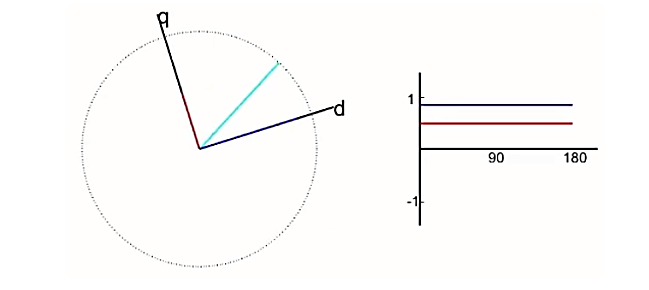
\includegraphics[width=12cm]{image18.png}
  \caption{Park Transform}
  \label{fig:image18}
\end{figure}

The Park Angle Transform block converts the alpha, beta, and zero components of Clarke Transformer in a stationary reference frame to direct, quadrature, and zero components in a rotating reference frame. For balanced three-phase systems, the zero components are equal to zero.

The Clarke to Park Angle Transform block implements the transform for an a-phase to q-axis alignment as

\begin{equation}
  \begin{bmatrix}
    d \\
    q \\
    0 \\
    \end{bmatrix} = \begin{bmatrix}
    \sin(\theta) & - \cos(\theta) & 0 \\
    \cos(\theta) & \sin(\theta) & 0 \\
    0 & 0 & 1 \\
    \end{bmatrix}\begin{bmatrix}
    \alpha \\
    \beta \\
    0 \\
    \end{bmatrix}
  \label{equation:eq11}
\end{equation}

where
\begin{itemize}
  \item \(\alpha \ and \ \beta\) are the components of the two-axis system in the stationary reference frame.
  \item 0 is the zero component of the two-axis system in the stationary reference frame.
  \item d and q are the direct-axis and quadrature-axis components of the two-axis system in the rotating reference frame.
\end{itemize}
%%%%%%%%%%%%%%%%%%%%%%%%%%%%%%%%%%%%%%%%%%%%%%%%%%%%%%%%%%%%%%%%%%%%%%%%%%%%%%%%%%%%%%%%%%%%

%%%%%%%%%%%%%%%%%%%%%%%%%%%%%%%%%%%%%%%%%%%%%%%%%%%%%%%%%%%%%%%%%%%%%%%%%%%%%%%%%%%%%%%%%%%%
\section{Filter Design}
As we are concerned about our health, we use water filters to purify the water. The same happens with electricity; there are impurities in it called harmonics, which are not wanted in our electrical systems. Harmonics affect electrical equipment, increasing its heat, reducing its lifetime and efficiency, and introducing noise to any system connected to the grid. These are just a few of the negativities of harmonics.

So, we use filters, which are devices that filter the frequency of electronic signals by manipulating the waves' amplitude and phase shift. As we know, the sine wave has its amplitude and phase shift, so anything outside the boundaries of its amplitude and phase shift is not desired and needs to be eliminated. This leads us to Fourier series, a mathematical theory that analyzes the signal into the fundamental wave and its harmonics.

There are two types of filters: active and passive. Not all filters are suitable for every application, and not all filters remove all harmonic frequencies. Therefore, we need to carefully choose the suitable filter for each application.
%%%%%%%%%%%%%%%%%%%%%%%%%%%%%%%%%%%%%%%%%%%%%%%%%%%%%%%%%%%%%%%%%%%%%%%%%%%%%%%%%%%%%%%%%%%%

%%%%%%%%%%%%%%%%%%%%%%%%%%%%%%%%%%%%%%%%%%%%%%%%%%%%%%%%%%%%%%%%%%%%%%%%%%%%%%%%%%%%%%%%%%%%
\subsection{Active Filters}
They are called active because they need an external power source to operate and are built of op-amps. The main advantage of these filters is that the output signals meet low resistance, allowing the signals to be amplified, and we can also control the gain's value to control the output signal amplitude. Some common types of active filters are low-pass filters, high-pass filters, band-pass filters, and band-stop filters.

These filters are used at low frequencies, so we cannot use inductors in active filters as we know that X\textsubscript{L} = 2\(\pi\)\emph{fL}. At low frequencies, the reactance would be extremely low, so the low-frequency harmonics would not be eliminated; we can say that they would not be noticed by the filter. Therefore, if there is an application or system that operates at low frequencies, it is more efficient to use active filters.
%%%%%%%%%%%%%%%%%%%%%%%%%%%%%%%%%%%%%%%%%%%%%%%%%%%%%%%%%%%%%%%%%%%%%%%%%%%%%%%%%%%%%%%%%%%%

%%%%%%%%%%%%%%%%%%%%%%%%%%%%%%%%%%%%%%%%%%%%%%%%%%%%%%%%%%%%%%%%%%%%%%%%%%%%%%%%%%%%%%%%%%%%
\subsection{Passive Filters}
They are used in high switching frequency systems because op-amps cannot manage this range of power and frequency and grid-connected systems. We need to cut the harmonics that accompany the current out of the grid as they are called passive, so they do not need an external power source to operate. We can logically estimate why these passive filters are very well used in grid-connected systems. We need to purify the signals out from the grid, so we cannot use them to supply the active filter. Therefore, we use passive filters. There are three types of passive filters: L, LC, and LCL filters. There are also two types, one called a trap filter and the other called a notch filter, but we are not interested in these types in this paper.
%%%%%%%%%%%%%%%%%%%%%%%%%%%%%%%%%%%%%%%%%%%%%%%%%%%%%%%%%%%%%%%%%%%%%%%%%%%%%%%%%%%%%%%%%%%%

%%%%%%%%%%%%%%%%%%%%%%%%%%%%%%%%%%%%%%%%%%%%%%%%%%%%%%%%%%%%%%%%%%%%%%%%%%%%%%%%%%%%%%%%%%%%
\subsubsection{L-type Filter}
The simplest and most widely used passive filter is the L-type filter, consisting of a single inductor connected in series with the inverter output. It offers low-pass filtering characteristics, effectively attenuating high-frequency harmonics while allowing fundamental frequency components to pass through. However, its effectiveness is limited to lower switching frequencies and may require larger inductors for higher power applications, leading to higher costs. This leads to LC and LCL filters.
%%%%%%%%%%%%%%%%%%%%%%%%%%%%%%%%%%%%%%%%%%%%%%%%%%%%%%%%%%%%%%%%%%%%%%%%%%%%%%%%%%%%%%%%%%%%

%%%%%%%%%%%%%%%%%%%%%%%%%%%%%%%%%%%%%%%%%%%%%%%%%%%%%%%%%%%%%%%%%%%%%%%%%%%%%%%%%%%%%%%%%%%%
\subsubsection{LC-type Filter}
An LC-type filter incorporates both an inductor (L) and a capacitor (C) in a series-parallel configuration. It supplies enhanced filtering performance compared to the L-type filter, offering a higher attenuation rate and broader harmonic suppression. However, its disadvantage, like the L-filter, is that at high switching frequencies, we need to use bulky inductors, leading to the same cost problem as before.
%%%%%%%%%%%%%%%%%%%%%%%%%%%%%%%%%%%%%%%%%%%%%%%%%%%%%%%%%%%%%%%%%%%%%%%%%%%%%%%%%%%%%%%%%%%%

%%%%%%%%%%%%%%%%%%%%%%%%%%%%%%%%%%%%%%%%%%%%%%%%%%%%%%%%%%%%%%%%%%%%%%%%%%%%%%%%%%%%%%%%%%%%
\subsubsection{LCL-type Filter}
The LCL-type filter is a more advanced filter topology, featuring two inductors (L) separated by a capacitor (C). It offers superior harmonic suppression and a lower resonant frequency compared to the LC-type filter, making it suitable for higher power applications and higher switching frequencies. However, its design is more complex, and its main disadvantage is that there is some instability in frequencies near the resonant frequency. Damping resistors are added in series or parallel to the capacitor to prevent resonance-related instability.
%%%%%%%%%%%%%%%%%%%%%%%%%%%%%%%%%%%%%%%%%%%%%%%%%%%%%%%%%%%%%%%%%%%%%%%%%%%%%%%%%%%%%%%%%%%%

%%%%%%%%%%%%%%%%%%%%%%%%%%%%%%%%%%%%%%%%%%%%%%%%%%%%%%%%%%%%%%%%%%%%%%%%%%%%%%%%%%%%%%%%%%%%
\subsection{Grid-Connected Inverters}
The main consideration in choosing between LC and LCL filters is whether the system is connected to the grid or not. Suppose we have an inverter connected to the grid, as in Figure \ref{fig:image19}. We cannot use an LC filter here.

\begin{figure}[h]
  \centering
  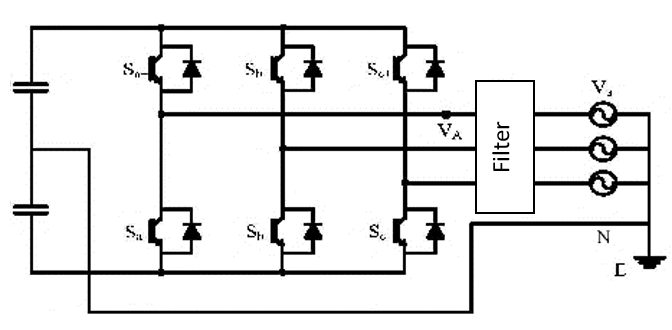
\includegraphics[width=15cm]{image19.png}
  \caption{Three-phase Inverter with Passive Filter}
  \label{fig:image19}
\end{figure}

If we use an LC filter, the capacitors would be considered capacitive loads to the grid, so the power factor (PF) would be leading. This means that the voltage across the capacitors would come before the grid's voltage, and the output current from the inverter would not pass through to the grid but would flow to the capacitors.

In high-frequency harmonics, the grid impedance is less than the capacitive reactance, so in an LC filter, the current will flow to the grid with harmonics. However, in the case of an LCL filter, the grid-connected inductor will block the current, and it will flow to the capacitors. Therefore, we use LCL filters in grid-connected inverters because of the tiny impedance of the grid, which causes a problem in high frequencies.

Here are some specific scenarios where an LCL filter would be a better choice than an LC filter:
\begin{itemize}
  \item Grid-connected inverters: LCL filters are commonly used in grid-connected inverters to attenuate harmonics and follow grid harmonics standards. The lower resonant frequency of LCL filters makes them less susceptible to resonances caused by the grid impedance.
  \item High-power applications: In high-power applications, the switching frequency of the power converter is often higher to reduce the size and weight of the inductors and capacitors. This higher switching frequency can lead to more harmonics, so an LCL filter is often necessary to supply adequate attenuation.
  \item Applications with a sensitive load: If the load is sensitive to harmonics, such as a motor or a computer system, an LCL filter can help to protect the load from damage.
\end{itemize}
%%%%%%%%%%%%%%%%%%%%%%%%%%%%%%%%%%%%%%%%%%%%%%%%%%%%%%%%%%%%%%%%%%%%%%%%%%%%%%%%%%%%%%%%%%%%

%%%%%%%%%%%%%%%%%%%%%%%%%%%%%%%%%%%%%%%%%%%%%%%%%%%%%%%%%%%%%%%%%%%%%%%%%%%%%%%%%%%%%%%%%%%%
\subsection{Method I}
This method discusses the empirical design of L filter. Note that this method is not based on any reference but practical experience in the field. L filter was extremely popular until IEEE 519- 1992 standards were introduced. Because to meet all the requirements in the standards, the L filter rating and size become remarkably high.

The following parameters are needed for the design: \emph{E\textsubscript{n}} -- Line to line RMS voltage (rectifier input), \emph{f\textsubscript{g}} -- grid frequency and \emph{S\textsubscript{rated}} -- apparent rated power. The base impedance is calculated using equation \ref{equation:eq12}
\begin{equation}
  Z_{b} = \ \frac{{E_{n}}^{2}}{S_{rated}}
  \label{equation:eq12}
\end{equation}

We can assume that the inductive reactance (\emph{X\textsubscript{L}}) is roughly around 5\% to 10\% of the base impedance. Thus, we can calculate the inductive reactance and the inductance using the following equations:
\begin{equation}
  X_{L} = (0.05\ to\ 0.1)Z_{b}
  \label{equation:eq13}
\end{equation}
where
\begin{equation}
  L = \ \frac{X_{L}}{2\pi f_{g}}
  \label{equation:eq14}
\end{equation}
The addition of a resistor in series with the inductor in an L filter is crucial for maintaining stability, protecting components, and complying with EMI standards in grid-connected inverter applications. This resistor value can be empirically calculated as third of the inductive reactance as shown in the following equation:
\begin{equation}
  R = \ \frac{\ X_{L}}{3}
  \label{equation:eq15}
\end{equation}
%%%%%%%%%%%%%%%%%%%%%%%%%%%%%%%%%%%%%%%%%%%%%%%%%%%%%%%%%%%%%%%%%%%%%%%%%%%%%%%%%%%%%%%%%%%%

%%%%%%%%%%%%%%%%%%%%%%%%%%%%%%%%%%%%%%%%%%%%%%%%%%%%%%%%%%%%%%%%%%%%%%%%%%%%%%%%%%%%%%%%%%%%
\subsubsection{Design Example}
A step-by-step procedure to obtain parameters of the filter with considering the following given data, needed for the filter design: \emph{E\textsubscript{n}} = 380V- line to line RMS voltage, \emph{P\textsubscript{rated}} = 1000W- rated active power, \emph{f\textsubscript{g}} = 50Hz-grid frequency. 

Considering a unity power factor system:
\[S_{rated} = \ P_{rated} = 1000VA\]
Therefore, the base impedance and the base capacitance are:
\[Z_{b} = \ \frac{380^{2}}{1000} = 144.4\mathrm{\Omega}\]
The filter inductive reactance can be calculated by:
\[X_{L} = 0.1*144.4 = 14.4\mathrm{\Omega}\]
To calculate the inductance:
\[L = \ \frac{14.4}{2\pi*50} = 45mH\]
Therefore, the resonant frequency satisfies the equation, and the damping resistance can be calculated as follows:
\[R = \ \frac{\ 14.4}{3} = 4.8\mathrm{\Omega}\]
%%%%%%%%%%%%%%%%%%%%%%%%%%%%%%%%%%%%%%%%%%%%%%%%%%%%%%%%%%%%%%%%%%%%%%%%%%%%%%%%%%%%%%%%%%%%

%%%%%%%%%%%%%%%%%%%%%%%%%%%%%%%%%%%%%%%%%%%%%%%%%%%%%%%%%%%%%%%%%%%%%%%%%%%%%%%%%%%%%%%%%%%%
\subsubsection{Simulation}
A simulation of method I was done on MATLAB-Simulink to check the performance of the system with the filter using the design example that was mentioned previously in that method. Here is the output voltage \emph{V\textsubscript{DC}}:

\begin{figure}[h!]
  \centering
  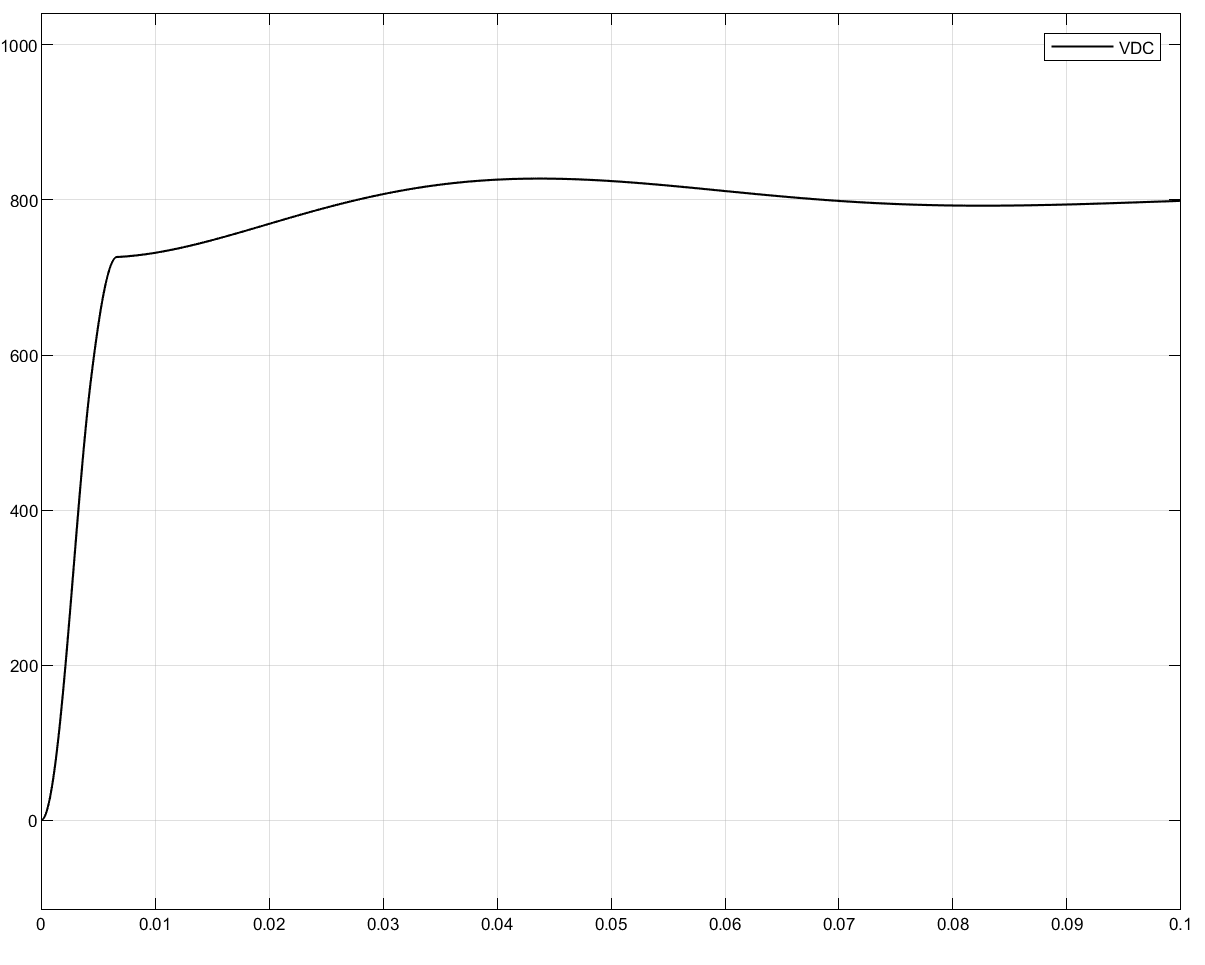
\includegraphics[width=11cm]{image20.png}
  \caption{The Output Voltage on The DC-Link on Simulink -- Method I}
  \label{fig:image20}
\end{figure}
Also, we had to check the phase shift between voltage and current of one of the phases as shown in Figure \ref{fig:image21}:

\begin{figure}[h!]
  \centering
  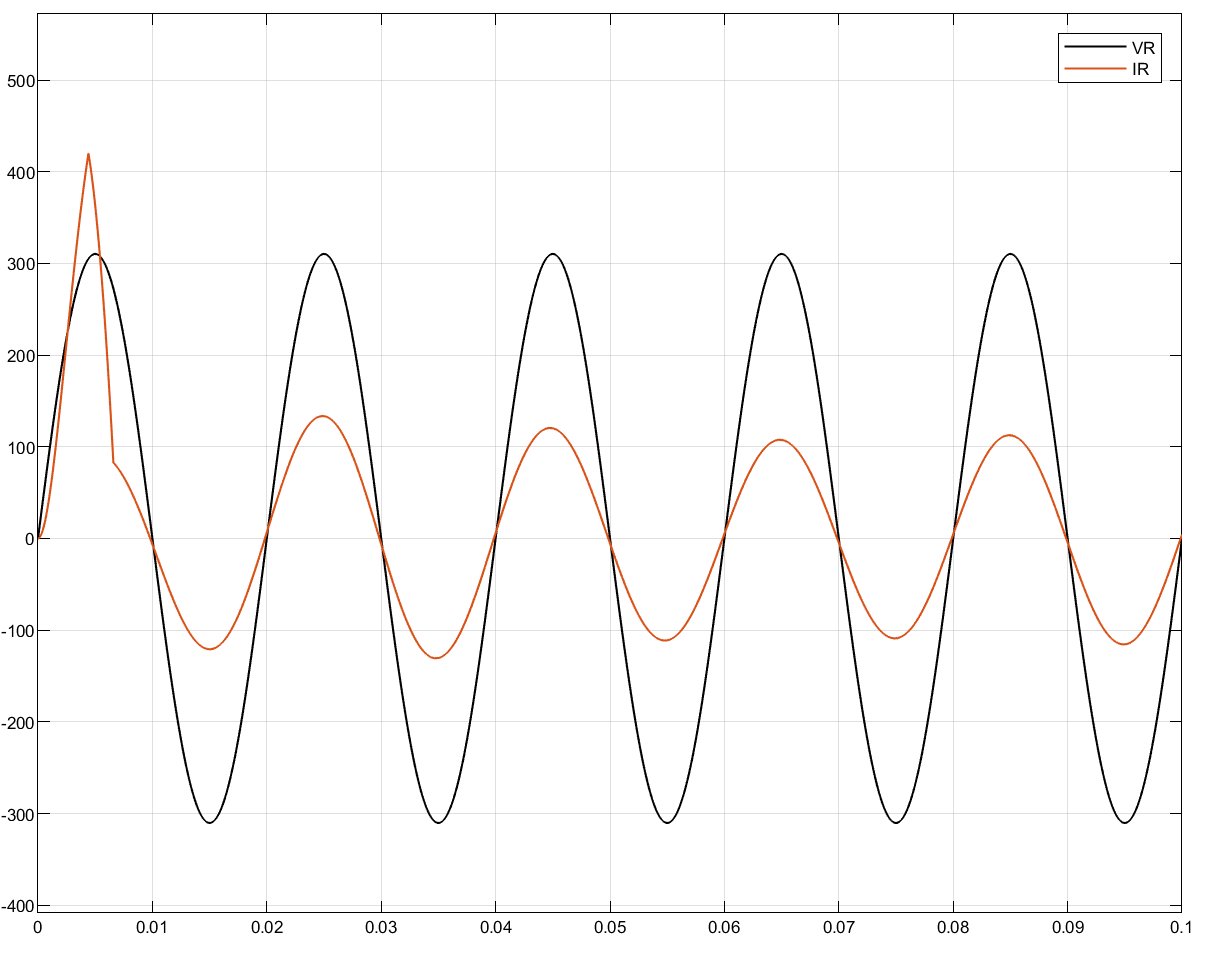
\includegraphics[width=11cm]{image21.png}
  \caption{The Current and The Phase Voltage of Phase R -- Method I}
  \label{fig:image21}
\end{figure}
Note that this is not the actual waveform of the current but a multiple of it. It was multiplied by fifty just so we can observe the two waveforms at the same time.
%%%%%%%%%%%%%%%%%%%%%%%%%%%%%%%%%%%%%%%%%%%%%%%%%%%%%%%%%%%%%%%%%%%%%%%%%%%%%%%%%%%%%%%%%%%%

%%%%%%%%%%%%%%%%%%%%%%%%%%%%%%%%%%%%%%%%%%%%%%%%%%%%%%%%%%%%%%%%%%%%%%%%%%%%%%%%%%%%%%%%%%%%
\subsection{Method II}
The design of LCL filters must consider several critical constraints, including current ripple, filter size, and switching ripple attenuation. As noted in \cite{lcl2012}, the reactive power variation introduced by the capacitor can cause resonance, potentially destabilizing the system. To address this issue, a damping mechanism, such as a resistor in serieswith the capacitor, is recommended.

This method meticulously outlines the LCL filter design process, emphasizing the importance of proper damping to prevent resonance. The algorithm for selecting LCL filter parameters utilizes the converter's power rating, grid frequency, and switching frequency as inputs.

The following parameters are needed for the design: \emph{E\textsubscript{n}} -- Line to line RMS voltage (rectifier input), \emph{V\textsubscript{ph}} -- phase voltage (rectifier input), \emph{P\textsubscript{n}} -- rated active power, \emph{V\textsubscript{DC}} -- DC bus voltage, \emph{f\textsubscript{g}} -- grid frequency, \emph{f\textsubscript{sw}} -- switching frequency and\emph{f\textsubscript{res}} -- resonance frequency.

The base impedance and base capacitance are defined by equations \ref{equation:eq16} and \ref{equation:eq17}. Thus, the filter values will be referred in \% of the base values:
\begin{equation}
  Z_{b} = \ \frac{{E_{n}}^{2}}{P_{n}}
  \label{equation:eq16}
\end{equation}
\begin{equation}
  C_{b} = \ \frac{1}{\omega_{n}Z_{b}}
  \label{equation:eq17}
\end{equation}
For the design of the filter capacitance, it is considered that the maximum power factor variation seen by the grid is 5\%, as it is multiplied by the value of base impedance of the system: \emph{C\textsubscript{f}} = 0.05\emph{C\textsubscript{b}}. where L\textsubscript{i} is inverter side inductor. A 10\% ripple of the rated current for the design parameters is given by:
\begin{equation}
  {\mathrm{\Delta}I}_{Lmax} = \ 0.1I_{\max}
  \label{equation:eq18}
\end{equation}
where
\begin{equation}
  I_{\max} = \ \frac{P_{n}\sqrt{2}}{{3V}_{ph}}
  \label{equation:eq19}
\end{equation}
\begin{equation}
  L_{i} = \ \frac{V_{DC}}{6f_{sw}{\mathrm{\Delta}I}_{Lmax}}
  \label{equation:eq20}
\end{equation}
The main objective of the LCL filter design is in fact to reduce the expected 10\% current ripple limit to 20\% of its own value, resulting in a ripple value of 2\% of the output current. To calculate the ripple reduction, the LCL filter equivalent circuit is first analyzed considering the inverter as a current source for each harmonic frequency.

The following equations give the relation between the harmonic current generated by the inverter and the once injected in the grid:
\begin{equation}
  L_{g} = \ \frac{\sqrt{\frac{1}{{K_{a}}^{2}}}\  + \ 1}{C_{f}{\omega_{sw}}^{2}}
  \label{equation:eq21}
\end{equation}
where, \emph{K\textsubscript{a}} is the desired attenuation.

A resistor in series (\emph{R\textsubscript{f}}) with the capacitor attenuates part of the ripple on the switching frequency to avoid the resonance. The value of this resistor should be one third of the impedance of the filter capacitor at the resonant frequency and the resistor in series with the filter capacitance is given by \ref{equation:eq24}.
\begin{equation}
  \omega_{res} = \ \sqrt{\frac{L_{i} + L_{g}}{L_{i}L_{g}C_{f}}}
  \label{equation:eq22}
\end{equation}
\begin{equation}
  {10f}_{g} < \ f_{res} < 0.5f_{sw}\ \
  \label{equation:eq23}
\end{equation}
It is necessary to check resonant frequency to satisfy \ref{equation:eq23}. If it does not, the parameters should be re-chosen.
\begin{equation}
  R_{f} = \ \frac{\ 1}{3\omega_{res}C_{f}}
  \label{equation:eq24}
\end{equation}
%%%%%%%%%%%%%%%%%%%%%%%%%%%%%%%%%%%%%%%%%%%%%%%%%%%%%%%%%%%%%%%%%%%%%%%%%%%%%%%%%%%%%%%%%%%%

%%%%%%%%%%%%%%%%%%%%%%%%%%%%%%%%%%%%%%%%%%%%%%%%%%%%%%%%%%%%%%%%%%%%%%%%%%%%%%%%%%%%%%%%%%%%
\subsubsection{Design Example}
A step-by-step procedure to obtain parameters of the filter with considering the following given data, needed for the filter design: \emph{E\textsubscript{n}} = 380V- line to line RMS voltage, \emph{V\textsubscript{ph}} = 220V- phase RMS voltage, \emph{P\textsubscript{n}} = 1000W- rated active power, \emph{V\textsubscript{DC}} = 800V- DC bus voltage, \emph{f\textsubscript{g}} = 50Hz-grid frequency, \emph{f\textsubscript{sw}} = 10KHz- switching frequency, \emph{K\textsubscript{a }}= 20\%- attenuation factor is done.

Therefore, the base impedance and the base capacitance are:
\[Z_{b} = \ \frac{380^{2}}{1000} = 144.4\mathrm{\Omega}\]
\[C_{b} = \ \frac{1}{2\pi*50*144.4} = 22\mathrm{\mu}F\]
The filter capacitance can be calculated by:
\[C_{f} = \ 0.05*22*10^{- 6} = 1.1\mathrm{\mu}F\]
To calculate the inverter-side inductor:
\[I_{\max} = \ \frac{1000\sqrt{2}}{3*220} = 2.14A\]
\[{\mathrm{\Delta}I}_{Lmax} = \ 0.1*2.14 = 0.214A\]
\[L_{i} = \ \frac{800}{6*10000*0.214} = 62.3mH\]
For the grid-side inductor:
\[L_{g} = \ \frac{\sqrt{\frac{1}{{0.2}^{2}}}\  + \ 1}{1.1*10^{- 6}{(2\pi*10000)}^{2}} = 1.38mH\]
Now, we shall check if the system is within the stable region to avoid resonance:
\[\omega_{res} = \ \sqrt{\frac{1.38*10^{- 3} + 62.3*10^{- 3}}{1.38*10^{- 3}*62.3*10^{- 3}*1.1*10^{- 6}}} = 25949rad\]
\[f_{res} = \ \frac{25949}{2\pi} = 4129.92Hz\]
\[10*50 < \ f_{res} < 0.5*10000\]
Therefore, the resonant frequency satisfies the equation, and the damping resistance can be calculated as follows:
\[R_{f} = \ \frac{\ 1}{3*2\pi*4129.92*1.1*10^{- 6}} = 11.68\mathrm{\Omega}\]
%%%%%%%%%%%%%%%%%%%%%%%%%%%%%%%%%%%%%%%%%%%%%%%%%%%%%%%%%%%%%%%%%%%%%%%%%%%%%%%%%%%%%%%%%%%%

%%%%%%%%%%%%%%%%%%%%%%%%%%%%%%%%%%%%%%%%%%%%%%%%%%%%%%%%%%%%%%%%%%%%%%%%%%%%%%%%%%%%%%%%%%%%
\subsubsection{Simulation}
A simulation of method II was done on MATLAB-Simulink to check the performance of the system with the filter using the design example that was mentioned previously in that method. Here is the output voltage \emph{V\textsubscript{DC}}:

\begin{figure}[h!]
  \centering
  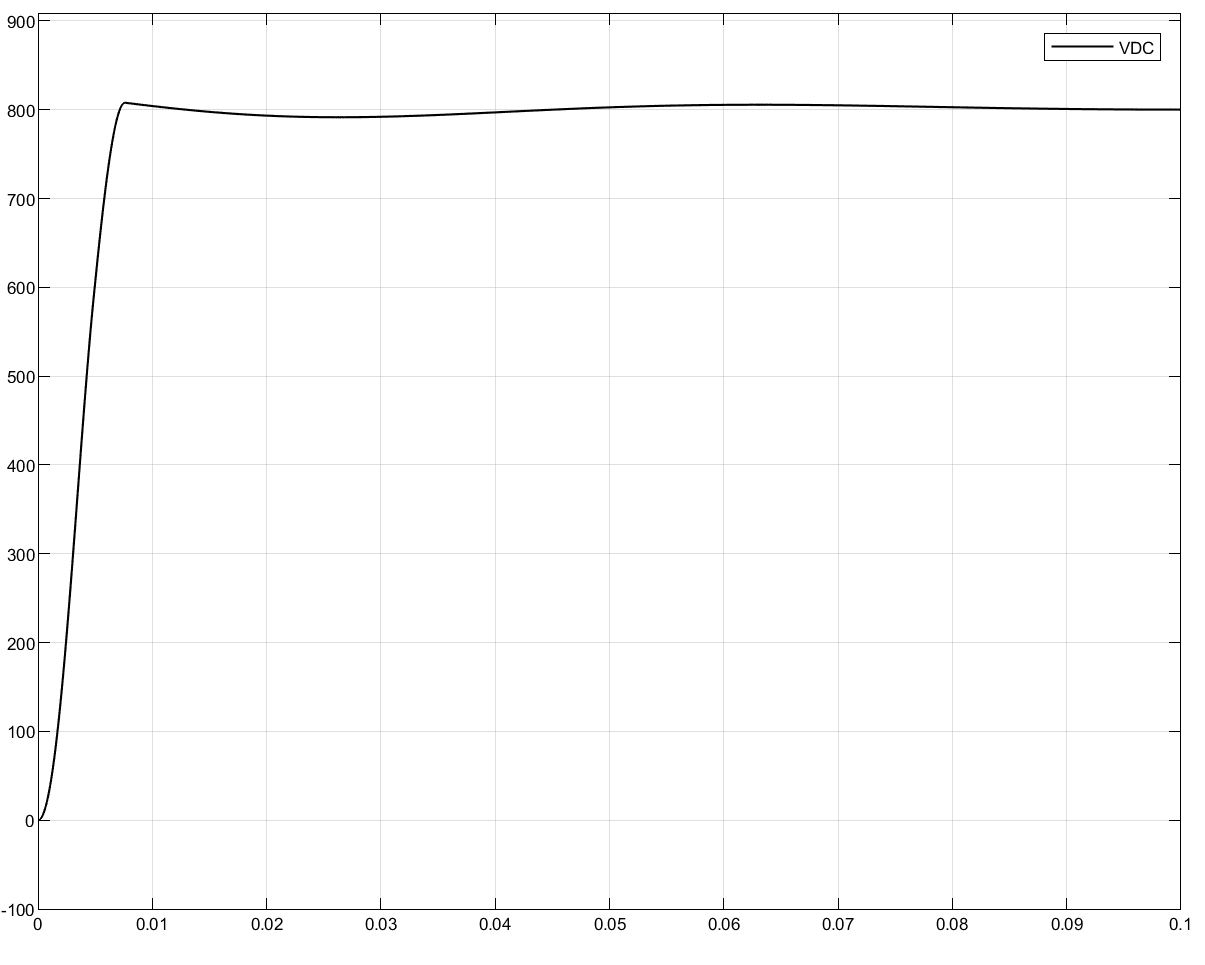
\includegraphics[width=11cm]{image22.png}
  \caption{The Output Voltage on The DC-Link on Simulink -- Method II}
  \label{fig:image22}
\end{figure}
Also, we had to check the phase shift between voltage and current of one of the phases as shown in Figure \ref{fig:image23}:

\begin{figure}[h!]
  \centering
  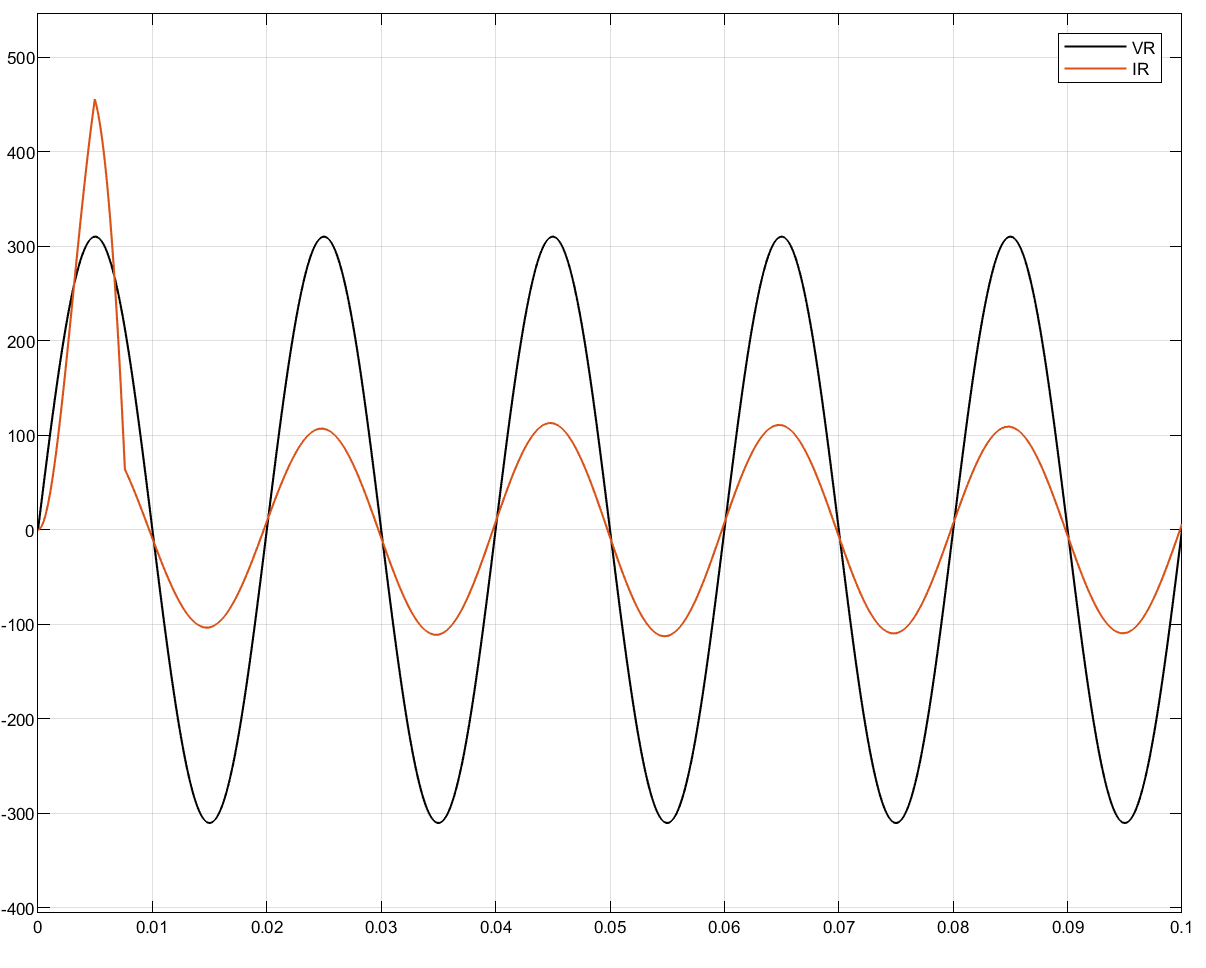
\includegraphics[width=11cm]{image23.png}
  \caption{The Current and The Phase Voltage of Phase R -- Method II}
  \label{fig:image23}
\end{figure}
Note that this is not the actual waveform of the current but a multiple of it. It was multiplied by fifty just so we can observe the two waveforms at the same time.
%%%%%%%%%%%%%%%%%%%%%%%%%%%%%%%%%%%%%%%%%%%%%%%%%%%%%%%%%%%%%%%%%%%%%%%%%%%%%%%%%%%%%%%%%%%%

%%%%%%%%%%%%%%%%%%%%%%%%%%%%%%%%%%%%%%%%%%%%%%%%%%%%%%%%%%%%%%%%%%%%%%%%%%%%%%%%%%%%%%%%%%%%
\subsection{Method III}
The design of LCL filters plays a crucial role in grid-connected inverter applications, ensuring efficient power transfer and minimizing harmonic distortion. This method, inspired by \cite{lcl2020}, provides a comprehensive framework for designing LCL filters that meet specific performance requirements while addressing potential stability issues. The method delves into the fundamental principles of LCL filter dynamics, enabling designers to make informed decisions about filter parameter selection.

To design the filter using this method, some parameters must be provided which are: \emph{S\textsubscript{rated}} -- apparent rated power, \emph{V\textsubscript{ph}} -- phase voltage (rectifier input), \emph{f\textsubscript{g}} -- grid frequency and \emph{f\textsubscript{sw}} -- switching frequency.

The filter capacitance is calculated at reactive power equals 5\% of the rated apparent power of the system. The reactive power is calculated as follows:
\begin{equation}
  Q_{rated} = \ C_{f}\omega_{n}{V_{ph}}^{2}
  \label{equation:eq25}
\end{equation}
where \(\omega\)\textsubscript{n} is the grid angular frequency. Therefore, the filter capacitance can be calculated according to equation \ref{equation:eq26}.
\begin{equation}
  C_{f} = \ \frac{0.05S_{rated}}{2\pi f_{g}{V_{ph}}^{2}}
  \label{equation:eq26}
\end{equation}
It is worth mentioning that the resonance frequency can be calculated as in the following equation:
\begin{equation}
  f_{res} = \ \frac{f_{sw}}{10}
  \label{equation:eq27}
\end{equation}
The value of the inverter-side inductor is selected based on the switching current. According to IEEE, the switching current is only 0.3\% of the rated grid current.
\begin{equation}
  I_{sw} = \ 0.003I_{grid}
  \label{equation:eq28}
\end{equation}
where
\begin{equation}
  I_{grid} = \ \frac{S_{rated}}{{3V}_{ph}}
  \label{equation:eq29}
\end{equation}
Now, for a triangular PWM scheme, minimum value of the switching voltage at switching frequency is 90\% of the grid phase voltage as shown in equation \ref{equation:eq30}.
\begin{equation}
  V_{sw} = \ 0.9V_{ph}
  \label{equation:eq30}
\end{equation}
Using the equations above inductance can be calculated as:
\begin{equation}
  L_{\min} = \frac{1}{|\omega_{sw}\frac{I_{sw}}{V_{sw}}\left( 1 - \frac{{\omega_{sw}}^{2}}{{\omega_{res}}^{2}} \right)|}
  \label{equation:eq31}
\end{equation}
Inverter-side inductor and grid-side inductor can be assumed to have the same value which is half of the calculated inductance (\emph{L\textsubscript{min}}).
\begin{equation}
  L_{g} = \ L_{i} = \frac{\ L_{\min}}{2}
  \label{equation:eq32}
\end{equation}
These are the minimum values of the required inductances. The maximum values are calculated based on the voltage drop across it. Voltage drop is always limited to 20\% of the grid phase voltage. So maximum inductance is given by:
\begin{equation}
  L_{\max} = \ \frac{0.2\ V_{ph}}{2\pi f_{g}I_{grid}}
  \label{equation:eq33}
\end{equation}
%%%%%%%%%%%%%%%%%%%%%%%%%%%%%%%%%%%%%%%%%%%%%%%%%%%%%%%%%%%%%%%%%%%%%%%%%%%%%%%%%%%%%%%%%%%%

%%%%%%%%%%%%%%%%%%%%%%%%%%%%%%%%%%%%%%%%%%%%%%%%%%%%%%%%%%%%%%%%%%%%%%%%%%%%%%%%%%%%%%%%%%%%
\subsubsection{Design Example}
To derive the parameters essential for filter design, follow these step-by-step procedures using the provided data: \emph{V\textsubscript{ph}} = 220V- phase RMS voltage, \emph{P\textsubscript{rated}} = 1000W- rated active power, \emph{f\textsubscript{g}} = 50Hz-grid frequency, \emph{f\textsubscript{sw}} = 10KHz- switching frequency.

Therefore, rated apparent power can be calculated as follow:
\[{S_{rated}}^{2} = \ {{(0.05S}_{rated})}^{2} + 1000^{2}\]
\[S_{rated} \cong 1000VA\]
To calculate the filter capacitance:
\[C_{f} = \ \frac{0.05*(\frac{1000}{3})}{2\pi*50*220^{2}} = 1.1\mu F\]
The resonance frequency is achieved by:
\[f_{res} = \ \frac{10000}{10} = 1000Hz\]
Calculating the minimum value of the inductance:
\[I_{grid} = \ \frac{1000}{3*220} = 1.51A\]
\[I_{sw} = \ 0.003*1.51 = 4.45mA\]
\[V_{sw} = \ 0.9*220 = 198V\]
\[L_{\min} = \frac{1}{|(2\pi*10000)\frac{4.45*10^{- 3}}{198}\left( 1 - \frac{{(2\pi*10000)}^{2}}{{(2\pi*1000)}^{2}} \right)|} = 7.15mH\]
So, the minimum value of the inverter-side and grid-side inductors is equal to:
\[L_{g} = \ L_{i} = \frac{7.15*10^{- 3}}{2} = 3.58mH\]
To get the maximum value of the inductance:
\[L_{\max} = \ \frac{0.2*220}{2\pi*50*1.51} = 92.75mH\]
The maximum value of the inverter-side and grid-side inductors is:
\[L_{g} = \ L_{i} = \frac{92.75*10^{- 3}}{2} = 46.37mH\]
%%%%%%%%%%%%%%%%%%%%%%%%%%%%%%%%%%%%%%%%%%%%%%%%%%%%%%%%%%%%%%%%%%%%%%%%%%%%%%%%%%%%%%%%%%%%

%%%%%%%%%%%%%%%%%%%%%%%%%%%%%%%%%%%%%%%%%%%%%%%%%%%%%%%%%%%%%%%%%%%%%%%%%%%%%%%%%%%%%%%%%%%%
\subsubsection{Simulation}
A simulation of method III was done on MATLAB-Simulink to check the performance of the system with the filter using the design example that was mentioned previously in that method. Here is the output voltage \emph{V\textsubscript{DC}}:

\begin{figure}[h!]
  \centering
  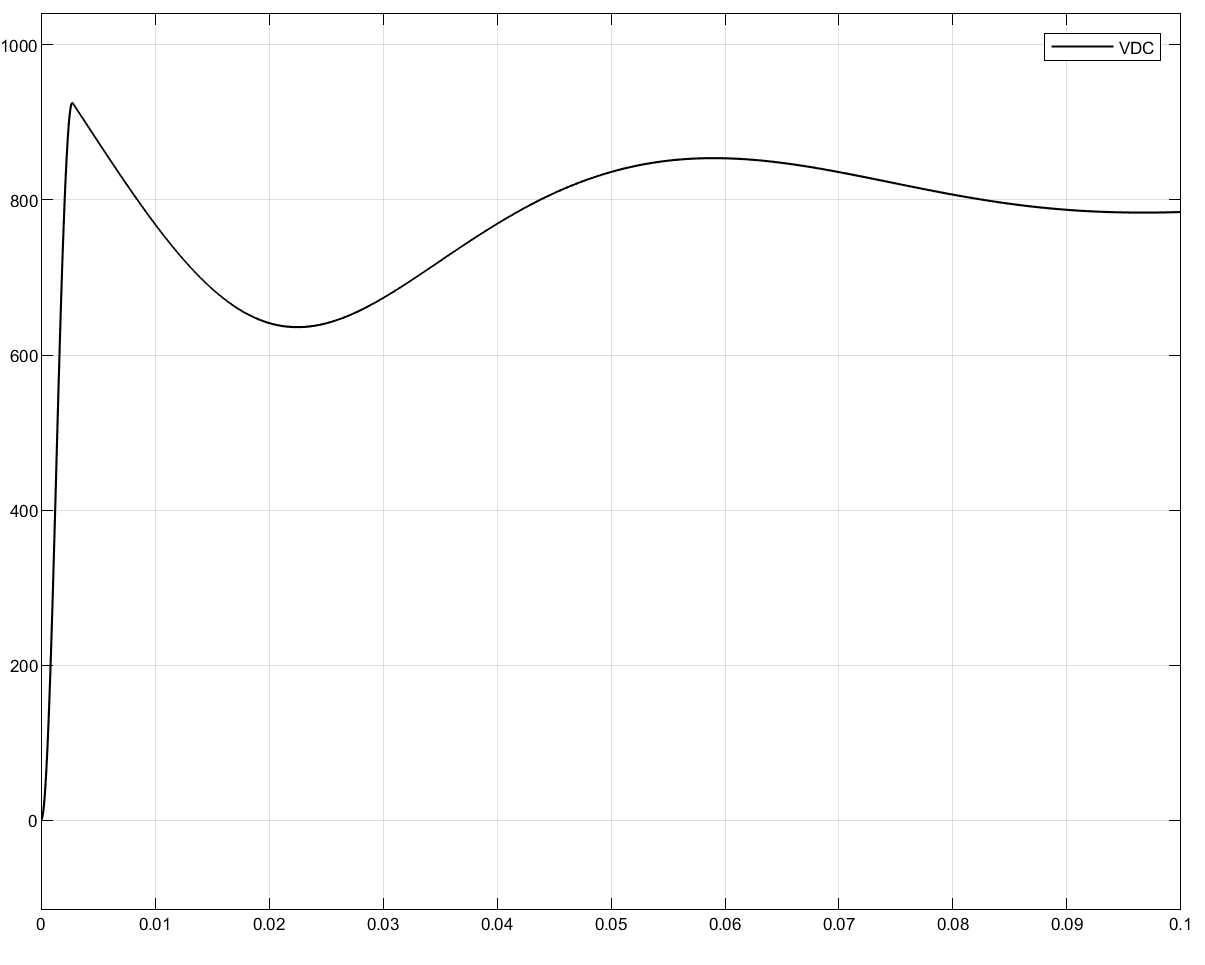
\includegraphics[width=11cm]{image26.png}
  \caption{The Output Voltage on The DC-Link on Simulink -- Method III}
  \label{fig:image26}
\end{figure}
Also, we had to check the phase shift between voltage and current of one of the phases as shown in Figure \ref{fig:image25}:

\begin{figure}[h!]
  \centering
  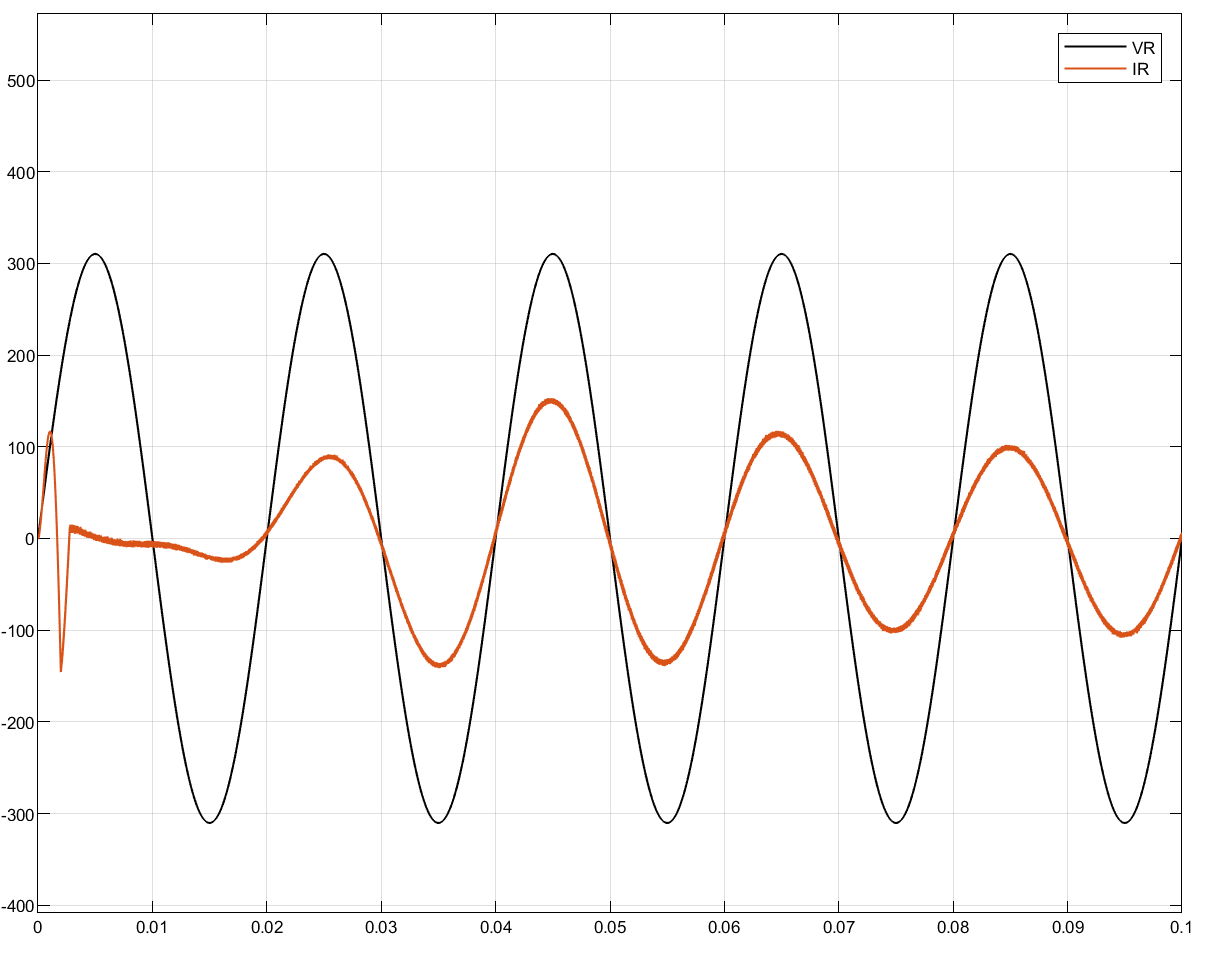
\includegraphics[width=11cm]{image27.png}
  \caption{The Current and The Phase Voltage of Phase R -- Method III}
  \label{fig:image27}
\end{figure}
Note that this is not the actual waveform of the current but a multiple of it. It was multiplied by fifty just so we can observe the two waveforms at the same time.
%%%%%%%%%%%%%%%%%%%%%%%%%%%%%%%%%%%%%%%%%%%%%%%%%%%%%%%%%%%%%%%%%%%%%%%%%%%%%%%%%%%%%%%%%%%%

%%%%%%%%%%%%%%%%%%%%%%%%%%%%%%%%%%%%%%%%%%%%%%%%%%%%%%%%%%%%%%%%%%%%%%%%%%%%%%%%%%%%%%%%%%%%
\subsection{Method IV}
This method according to \cite{lcl2010} deals with a design method of LCL filter for grid-connected three-phase inverters. By analyzing total harmonic distortion of the current (THD\textsubscript{i}) in the inverter-side inductor and the ripple attenuation factor of the current (RAF) injected to the grid through the LCL network, the parameter of LCL can be clearly designed.

The base impedance of the system must be known before choosing the LCL filter parameters. The base values of the impedance, inductance, and capacitance are defined as in equations \ref{equation:eq34} ~ \ref{equation:eq36}.
\begin{equation}
  Z_{b} = \ \frac{{E_{n}}^{2}}{P_{n}}
  \label{equation:eq34}
\end{equation}
\begin{equation}
  L_{b} = \ \frac{Z_{b}}{\omega_{n}}
  \label{equation:eq35}
\end{equation}
\begin{equation}
  C_{b} = \ \frac{1}{\omega_{n}Z_{b}}
  \label{equation:eq36}
\end{equation}
The inductance of inverter-side inductor is obtained by setting THD\textsubscript{i} within 10\% to 30\%. If THD\textsubscript{i} is set below 10\%, the inductance is increased, and the resonant frequency decreases. If THD\textsubscript{i} is increased more than 30\%, the resonant frequency increases. The resonant frequency should be set between the bandwidth of the controller and switching frequency.
\begin{equation}
  L_{i} = \ \frac{f_{g}}{f_{sw}} \times \frac{L_{b}}{{THD}_{i}} \times \sqrt{\frac{\pi^{2}}{18} \times \left( \frac{3}{2} - \frac{4\sqrt{3}}{\pi}m_{a} + \frac{9}{8}{m_{a}}^{2} \right)}
  \label{equation:eq37}
\end{equation}
where \emph{m\textsubscript{a}} is the modulation index.
\begin{equation}
  m_{a} = \ \frac{V_{ph}2\sqrt{2}}{V_{DC}}
  \label{equation:eq38}
\end{equation}
Filter capacitance must be set properly by setting x less than 5\% of base capacitance as follows:
\begin{equation}
  C_{f} \leq \ x\frac{1}{\omega_{n}Z_{b}}
  \label{equation:eq39}
\end{equation}
Use equation \ref{equation:eq40} to extract the grid-side inductance. After setting proper RAF, calculate the grid-side inductance.
\begin{equation}
  L_{g} = \ \frac{RAF + \ 1}{{RAFC}_{f}{\omega_{sw}}^{2}}
  \label{equation:eq40}
\end{equation}
Make sure the total inductance of inductor which is sum of the inductance of inverter-side inductor and grid-side inductor is less than 10\% of the base value of the inductance.
%%%%%%%%%%%%%%%%%%%%%%%%%%%%%%%%%%%%%%%%%%%%%%%%%%%%%%%%%%%%%%%%%%%%%%%%%%%%%%%%%%%%%%%%%%%%

%%%%%%%%%%%%%%%%%%%%%%%%%%%%%%%%%%%%%%%%%%%%%%%%%%%%%%%%%%%%%%%%%%%%%%%%%%%%%%%%%%%%%%%%%%%%
\subsubsection{Design Example}
A step-by-step procedure to obtain parameters of the filter with considering the following given data, needed for the filter design: \emph{E\textsubscript{n}} = 380V- line to line RMS voltage, \emph{V\textsubscript{ph}} = 220V- phase RMS voltage, \emph{P\textsubscript{n}} = 1000W- rated active power, \emph{V\textsubscript{DC}} = 800V- DC bus voltage, \emph{f\textsubscript{g}} = 50Hz-grid frequency, \emph{f\textsubscript{sw}} = 10KHz- switching frequency, \emph{THD\textsubscript{i}} = 20\%- total harmonic distortion of the current, \emph{RAF} = 20\%- attenuation factor is done. 

Therefore, the base impedance and the base capacitance are:
\[Z_{b} = \ \frac{380^{2}}{1000} = 144.4\mathrm{\Omega}\]
\[L_{b} = \ \frac{144.4}{2\pi*50} = 0.4596H\]
\[C_{b} = \ \frac{1}{2\pi*50*144.4} = 22\mu F\]
The filter capacitance can be calculated by:
\[C_{f} \leq \ 0.05*22*10^{- 6} = 1.1\mu F\]
The modulation index is as follows:
\[m_{a} = \ \frac{220*2\sqrt{2}}{800} = 0.778\]
To calculate the inverter-side inductor:
\[L_{i} = \ \frac{50}{10000} \times \frac{0.4596}{0.2} \times \sqrt{\frac{\pi^{2}}{18} \times \left( \frac{3}{2} - \frac{4\sqrt{3}}{\pi}*0.778 + \frac{9}{8}{(0.778)}^{2} \right)} = 5.8mH\]
For the grid-side inductor:
\[L_{g} = \ \frac{0.2 + \ 1}{0.2*1.1*10^{- 6}{(2\pi*10000)}^{2}} = 1.38mH\]
To make sure the design is correct:
\[L_{g} + L_{i} < 0.1L_{b}\]
\[1.38*10^{- 3} + 5.8*10^{- 3} < 0.1*0.4596\]
Therefore, the filter is well designed.
%%%%%%%%%%%%%%%%%%%%%%%%%%%%%%%%%%%%%%%%%%%%%%%%%%%%%%%%%%%%%%%%%%%%%%%%%%%%%%%%%%%%%%%%%%%%

%%%%%%%%%%%%%%%%%%%%%%%%%%%%%%%%%%%%%%%%%%%%%%%%%%%%%%%%%%%%%%%%%%%%%%%%%%%%%%%%%%%%%%%%%%%%
\subsubsection{Simulation}
A simulation of method IV was done on MATLAB-Simulink to check the performance of the system with the filter using the design example that was mentioned previously in that method. Here is the output voltage \emph{V\textsubscript{DC}}:

\begin{figure}[h!]
  \centering
  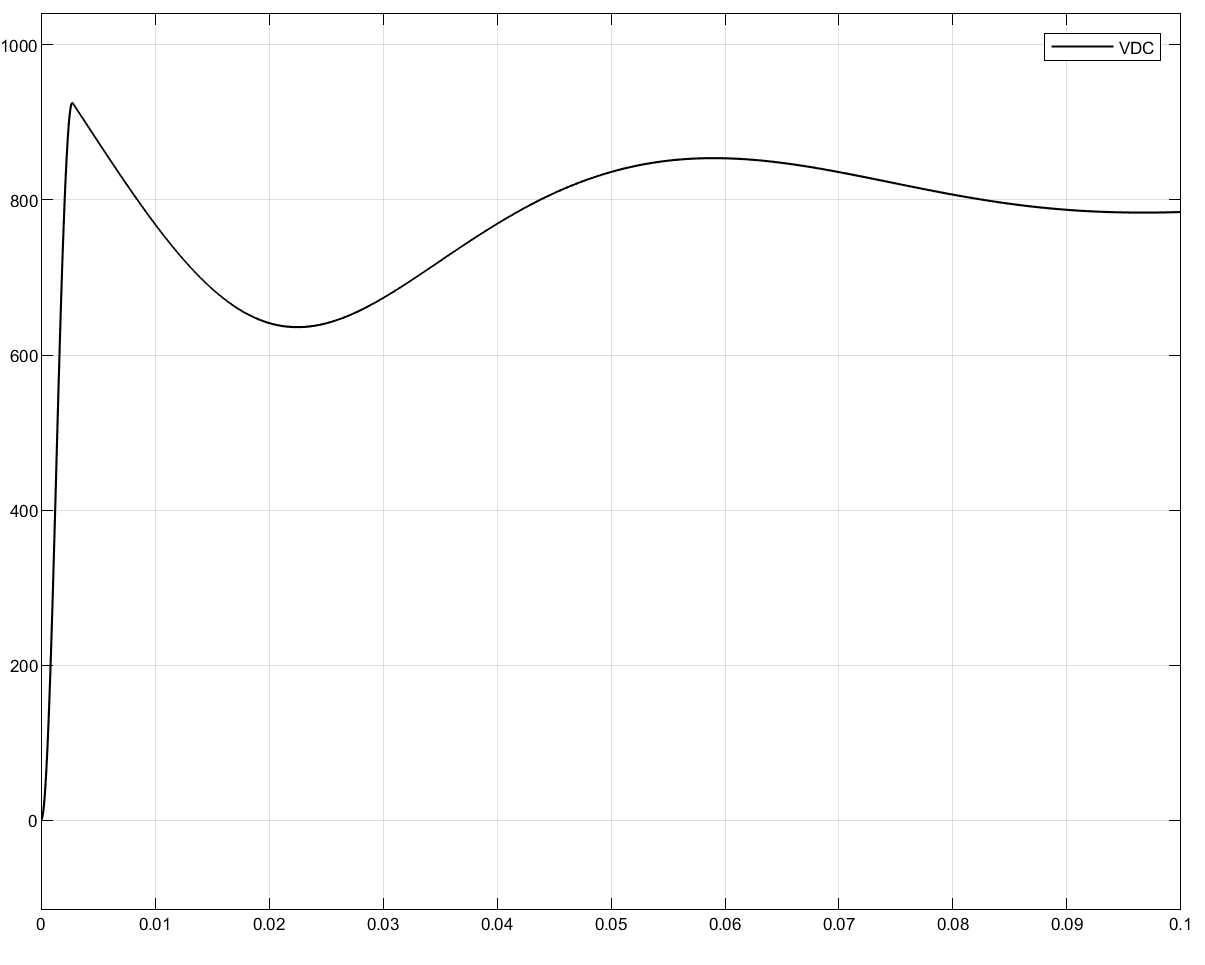
\includegraphics[width=11cm]{image26.png}
  \caption{The Output Voltage on The DC-Link on Simulink -- Method IV}
  \label{fig:image26}
\end{figure}
Also, we had to check the phase shift between voltage and current of one of the phases as shown in Figure \ref{fig:image27}:

\begin{figure}[h!]
  \centering
  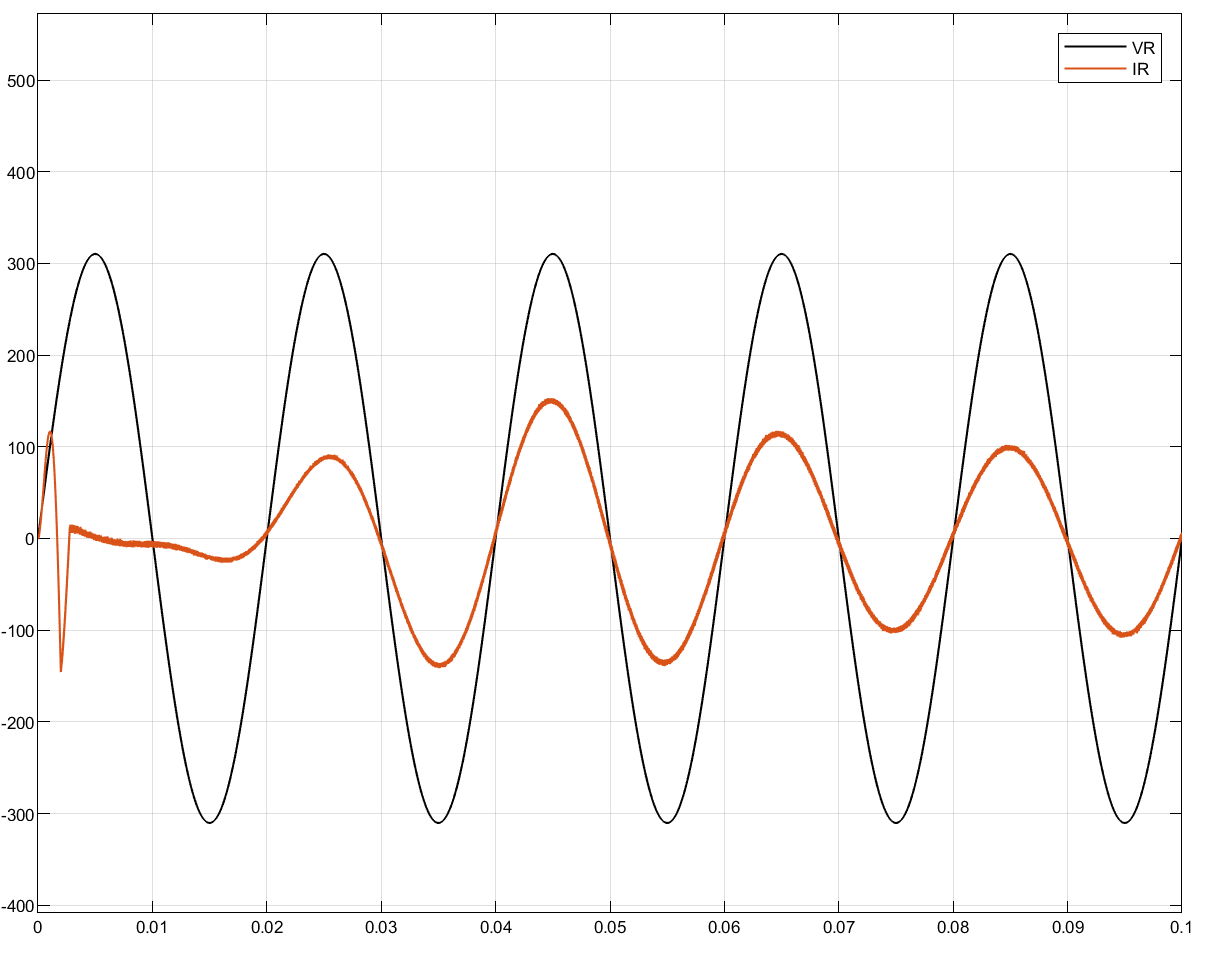
\includegraphics[width=11cm]{image27.png}
  \caption{The Current and The Phase Voltage of Phase R -- Method IV}
  \label{fig:image27}
\end{figure}
Note that this is not the actual waveform of the current but a multiple of it. It was multiplied by fifty just so we can observe the two waveforms at the same time.
%%%%%%%%%%%%%%%%%%%%%%%%%%%%%%%%%%%%%%%%%%%%%%%%%%%%%%%%%%%%%%%%%%%%%%%%%%%%%%%%%%%%%%%%%%%%

%%%%%%%%%%%%%%%%%%%%%%%%%%%%%%%%%%%%%%%%%%%%%%%%%%%%%%%%%%%%%%%%%%%%%%%%%%%%%%%%%%%%%%%%%%%%
\subsection{Method V}
The design of LCL filter can also be done via MATLAB code that was mentioned in \cite{lcl2014}. You may enter the system inputs like: \emph{P\textsubscript{n}} -- active rated power, \emph{V\textsubscript{ph}} -- phase voltage (rectifier input), \emph{V\textsubscript{DC}} -- DC bus voltage, \emph{f\textsubscript{n}} -- grid frequency and \emph{f\textsubscript{sw}} -- switching frequency.

It is worth mentioning that the code that is present in \cite{lcl2014} is for a single-phase grid-connected inverter but some of the data was changed to suit the three-phase grid-connected inverter, which is our case.
%%%%%%%%%%%%%%%%%%%%%%%%%%%%%%%%%%%%%%%%%%%%%%%%%%%%%%%%%%%%%%%%%%%%%%%%%%%%%%%%%%%%%%%%%%%%

%%%%%%%%%%%%%%%%%%%%%%%%%%%%%%%%%%%%%%%%%%%%%%%%%%%%%%%%%%%%%%%%%%%%%%%%%%%%%%%%%%%%%%%%%%%%
\subsubsection{Design Example}
To derive the parameters essential for filter design, follow these step-by-step procedures using the provided data: \emph{V\textsubscript{ph}} = 220V- phase RMS voltage, \emph{P\textsubscript{rated}} = 1000W- rated active power, \emph{f\textsubscript{g}} = 50Hz-grid frequency, \emph{f\textsubscript{sw}} = 10KHz- switching frequency, r = 0.6.

Therefore, the MATLAB code is as follows:
\begin{lstlisting}[language=Matlab, label=lst:matlabcode]
  % System parameters
  Pn = 1000; % Inverter power
  Vph = 220; %Grid phase RMS voltage
  Vdc=800; %DC link voltage
  fn = 50; %Grid frequency
  fsw = 10000; %Switching frequency
  
  En = Vph*sqrt(3);
  wn = 2*pi*fn;
  wsw = 2*pi*fsw;
  
  % Base values
  Zb = (En\^{}2)/Pn
  Cb = 1/(wn*Zb)

  % Filter parameters
  delta\_Ilmax=0.1*((Pn*sqrt(2))/(3*Vph))
  Li=Vdc/(8*fsw*delta\_Ilmax) %Inverter side inductance
  x = 0.05;
  Cf = x*Cb %Filter capacitor

  % Calculation of r,between Linv and Lg
  r = 0.6;

  % Grid side inductance
  Lg = r*Li

  % Calculation of frequency of the filter
  wres = sqrt((Li+Lg)/(Li*Lg*Cf));
  fres=wres/(2*pi)
  
  %Damping resistance
  Rd = 1/(3*wres*Cf)
\end{lstlisting}
And the LCL filter parameters as the output values of the code are as follow:
\[C_{f} = 1.1\mu F\]
\[L_{i} = \ 46.7mH\]
\[L_{g} = \ 28mH\]
\[R_{f} = \ 42.11\mathrm{\Omega}\]
%%%%%%%%%%%%%%%%%%%%%%%%%%%%%%%%%%%%%%%%%%%%%%%%%%%%%%%%%%%%%%%%%%%%%%%%%%%%%%%%%%%%%%%%%%%%

%%%%%%%%%%%%%%%%%%%%%%%%%%%%%%%%%%%%%%%%%%%%%%%%%%%%%%%%%%%%%%%%%%%%%%%%%%%%%%%%%%%%%%%%%%%%
\subsubsection{Simulation}
A simulation of method V was done on MATLAB-Simulink to check the performance of the system with the filter using the design example that was mentioned previously in that method. Here is the output voltage \emph{V\textsubscript{DC}}:

\begin{figure}[h!]
  \centering
  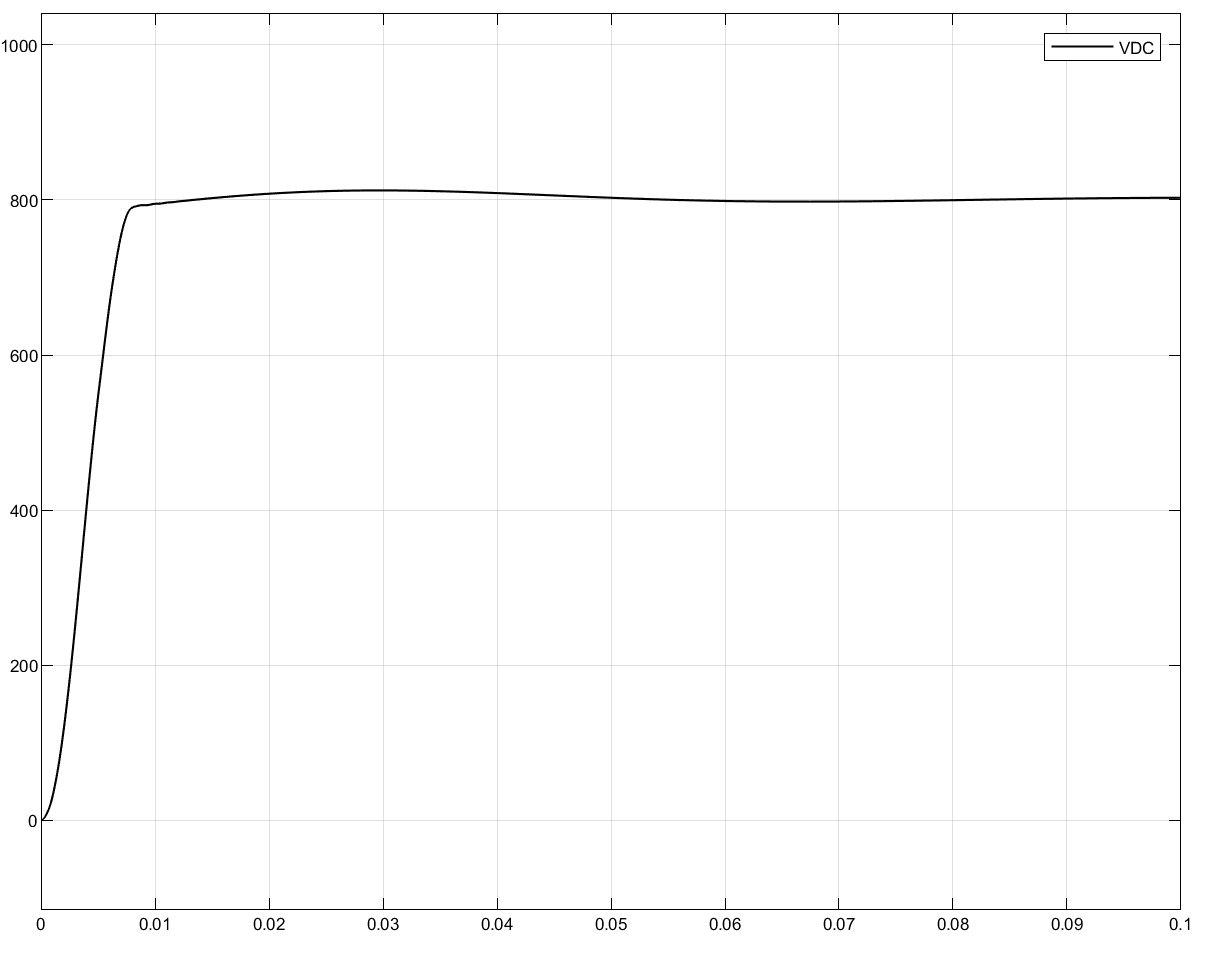
\includegraphics[width=11cm]{image28.png}
  \caption{The Output Voltage on The DC-Link on Simulink -- Method V}
  \label{fig:image28}
\end{figure}
Also, we had to check the phase shift between voltage and current of one of the phases as shown in Figure \ref{fig:image29}:

\begin{figure}[h!]
  \centering
  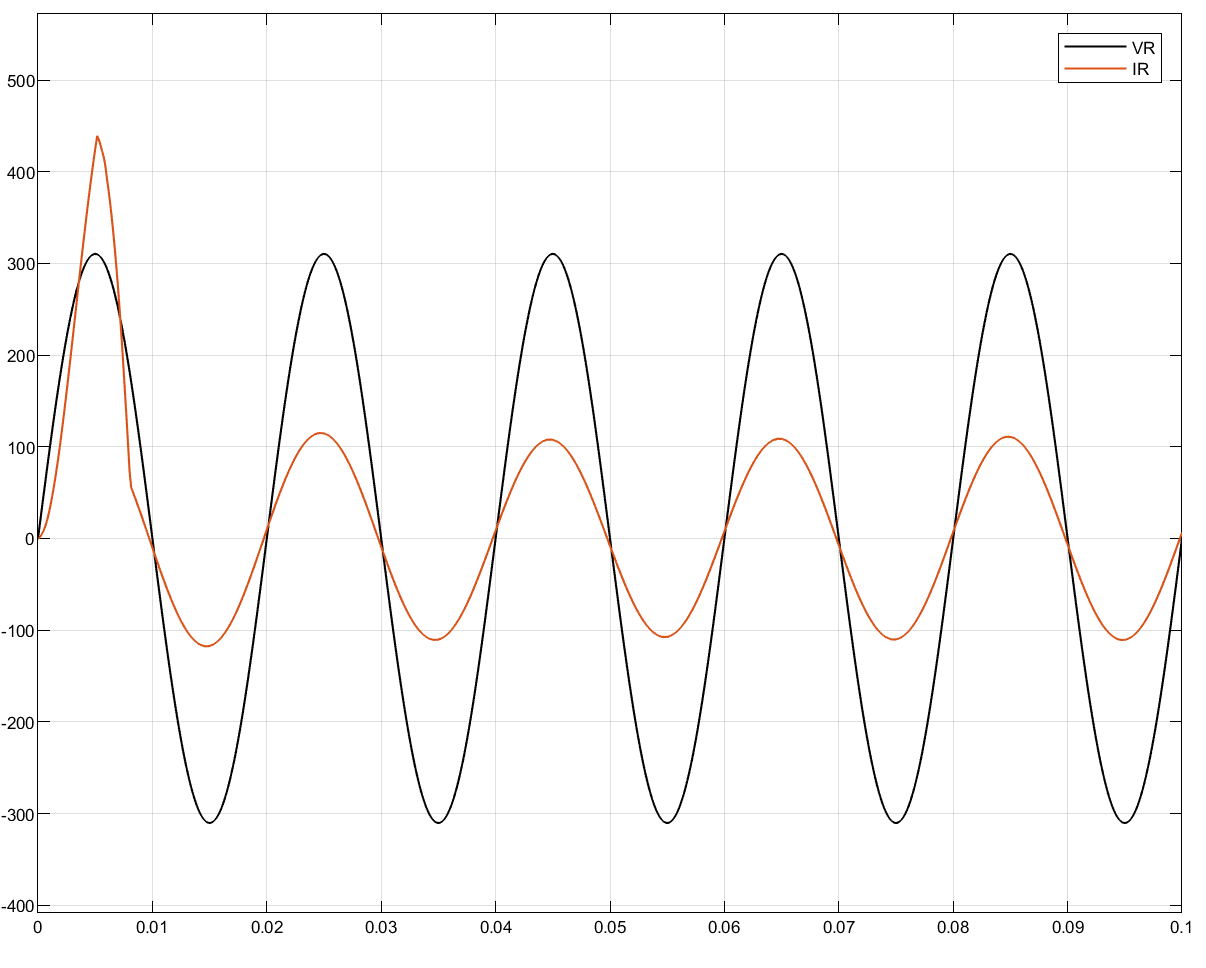
\includegraphics[width=11cm]{image29.png}
  \caption{The Current and The Phase Voltage of Phase R -- Method V}
  \label{fig:image29}
\end{figure}
Note that this is not the actual waveform of the current but a multiple of it. It was multiplied by fifty just so we can observe the two waveforms at the same time.
%%%%%%%%%%%%%%%%%%%%%%%%%%%%%%%%%%%%%%%%%%%%%%%%%%%%%%%%%%%%%%%%%%%%%%%%%%%%%%%%%%%%%%%%%%%%

%%%%%%%%%%%%%%%%%%%%%%%%%%%%%%%%%%%%%%%%%%%%%%%%%%%%%%%%%%%%%%%%%%%%%%%%%%%%%%%%%%%%%%%%%%%%
\subsection{Comparison}
After discussing multiple methods, it is now time to compare the output of each method. The following table contains the output of each method.

\begin{table}[h!]
  \centering
  \begin{tabular}{p{3.5cm} p{3.5cm} p{3.5cm} p{3.5cm}} 
   \hline
   $Method$ & $L\textsubscript{i}$ (mH) & $L\textsubscript{g}$ (mH) & $C\textsubscript{f}$ (\(\mu\)F) \\ [0.5ex] 
   \hline
   Method I & 45 & - & - \\
   Method II & 62.3 & 1.38 & 1.1 \\
   Method III & 3.58 -- 46.37 & 3.58 -- 46.37 & 1.1 \\
   Method IV & 5.8 & 1.38 & 1.1 \\
   Method V & 46.7 & 28 & 1.1 \\[1ex] 
   \hline
  \end{tabular}
  \caption{Comparison between The Output of Different Design Methods}
\end{table}
After learning all the different methods, each method shall be considered carefully to get the optimum output for the desired system. In our case, we have done multiple simulations to notice the output of each method. It was observed that each method produced the same output with slight differences. 

Yet, Method IV had the worst output as the phase current was full of ripples even by substituting by different values of inductance within the calculated range, also the output voltage had the highest settling time.

Method II and method V had the lowest overshot compared to the rest in this specific case, but method V had a smoother output. But at higher power (10k watt), method II had a way better response than method V leading it to be our preferred method. The PI controllers were calibrated in a way to have a leading power factor of 0.9998 with settling time of less than a half cycle with settling error of 0.5\%. Also, the second method’s design was checked by equation \ref{equation:eq23}, to make sure that the design would avoid resonance problems. 
%%%%%%%%%%%%%%%%%%%%%%%%%%%%%%%%%%%%%%%%%%%%%%%%%%%%%%%%%%%%%%%%%%%%%%%%%%%%%%%%%%%%%%%%%%%%

%%%%%%%%%%%%%%%%%%%%%%%%%%%%%%%%%%%%%%%%%%%%%%%%%%%%%%%%%%%%%%%%%%%%%%%%%%%%%%%%%%%%%%%%%%%%
\subsection{Chosen Method}
Two designs were done based on method II for both the low-rating system (1kW) and the high-rating system (10kW) to check its output.
%%%%%%%%%%%%%%%%%%%%%%%%%%%%%%%%%%%%%%%%%%%%%%%%%%%%%%%%%%%%%%%%%%%%%%%%%%%%%%%%%%%%%%%%%%%%

%%%%%%%%%%%%%%%%%%%%%%%%%%%%%%%%%%%%%%%%%%%%%%%%%%%%%%%%%%%%%%%%%%%%%%%%%%%%%%%%%%%%%%%%%%%%
\subsubsection{Design Example - Low Power}
A step-by-step procedure to obtain parameters of the filter with considering the following given data, needed for the filter design: \emph{E\textsubscript{n}} = 100V- line to line RMS voltage, \emph{V\textsubscript{ph}} = 57.73V- phase RMS voltage, \emph{P\textsubscript{n}} = 1000W- rated active power, \emph{V\textsubscript{DC}} = 200V- DC bus voltage, \emph{f\textsubscript{g}} = 50Hz-grid frequency, \emph{f\textsubscript{sw}} = 10KHz- switching frequency, \emph{K\textsubscript{a }}= 20\%- attenuation factor is done.

Therefore, the base impedance and the base capacitance are:
\[Z_{b} = \ \frac{100^{2}}{1000} = 10\mathrm{\Omega}\]
\[C_{b} = \ \frac{1}{2\pi*50*10} = 3.18*10^{- 4}F\]
The filter capacitance can be calculated by:
\[C_{f} = \ 0.05*3.18*10^{- 4} = 15.915\mu F\]
To calculate the inverter-side inductor:
\[I_{\max} = \ \frac{1000\sqrt{2}}{3*57.73} = 8.16A\]
\[{\mathrm{\Delta}I}_{Lmax} = \ 0.1*8.16 = 0.816A\]
\[L_{i} = \ \frac{200}{6*10000*0.816} = 4mH\]
For the grid-side inductor:
\[L_{g} = \ \frac{\sqrt{\frac{1}{{0.2}^{2}}}\  + \ 1}{15.915*10^{- 6}{(2\pi*10000)}^{2}} = 95.492uH\]
Now, we shall check if the system is within the stable region to avoid resonance:
\[\omega_{res} = \ \sqrt{\frac{4*10^{- 3} + 95*10^{- 6}}{4*10^{- 3}*95*10^{- 6}*15.915*10^{- 6}}} = 25952.26rad\]
\[f_{res} = \ \frac{25952.26}{2\pi} = 4130.4Hz\]
\[10*50 < \ f_{res} < 0.5*10000\]
Therefore, the resonant frequency satisfies the equation, and the damping resistance can be calculated as follows:
\[R_{f} = \ \frac{\ 1}{3*2\pi*4130.4*16*10^{- 6}} = 0.8027\mathrm{\Omega}\]
%%%%%%%%%%%%%%%%%%%%%%%%%%%%%%%%%%%%%%%%%%%%%%%%%%%%%%%%%%%%%%%%%%%%%%%%%%%%%%%%%%%%%%%%%%%%

%%%%%%%%%%%%%%%%%%%%%%%%%%%%%%%%%%%%%%%%%%%%%%%%%%%%%%%%%%%%%%%%%%%%%%%%%%%%%%%%%%%%%%%%%%%%
\subsubsection{Design Example - High Power}
A step-by-step procedure to obtain parameters of the filter with considering the following given data, needed for the filter design: \emph{E\textsubscript{n}} = 380V- line to line RMS voltage, \emph{V\textsubscript{ph}} = 220V- phase RMS voltage, \emph{P\textsubscript{n}} = 10KW- rated active power, \emph{V\textsubscript{DC}} = 800V- DC bus voltage, \emph{f\textsubscript{g}} = 50Hz-grid frequency, \emph{f\textsubscript{sw}} = 10KHz- switching frequency, \emph{K\textsubscript{a }}= 20\%- attenuation factor is done.

Therefore, the base impedance and the base capacitance are:
\[Z_{b} = \ \frac{380^{2}}{10000} = 14.44\mathrm{\Omega}\]
\[C_{b} = \ \frac{1}{2\pi*50*14.44} = 220\mu F\]
The filter capacitance can be calculated by:
\[C_{f} = \ 0.05*22*10^{- 6} = 11µF\]
To calculate the inverter-side inductor:
\[I_{\max} = \ \frac{10000\sqrt{2}}{3*220} = 21.4A\]
\[{\mathrm{\Delta}I}_{Lmax} = \ 0.1*21.4 = 2.14A\]
\[L_{i} = \ \frac{800}{6*10000*2.14} = 6.23mH\]
For the grid-side inductor:
\[L_{g} = \ \frac{\sqrt{\frac{1}{{0.2}^{2}}}\  + \ 1}{11*10^{- 6}{(2\pi*10000)}^{2}} = 0.138mH\]
Now, we shall check if the system is within the stable region to avoid resonance:
\[\omega_{res} = \ \sqrt{\frac{0.138*10^{- 3} + 6.23*10^{- 3}}{0.138*10^{- 3}*6.23*10^{- 3}*11*10^{- 6}}} = 25949rad\]
\[f_{res} = \ \frac{25949}{2\pi} = 4129.92Hz\]
\[10*50 < \ f_{res} < 0.5*10000\]
Therefore, the resonant frequency satisfies the equation, and the damping resistance can be calculated as follows:
\[R_{f} = \ \frac{\ 1}{3*2\pi*4129.92*11*10^{- 6}} = 1.168\mathrm{\Omega}\]
%%%%%%%%%%%%%%%%%%%%%%%%%%%%%%%%%%%%%%%%%%%%%%%%%%%%%%%%%%%%%%%%%%%%%%%%%%%%%%%%%%%%%%%%%%%%

%%%%%%%%%%%%%%%%%%%%%%%%%%%%%%%%%%%%%%%%%%%%%%%%%%%%%%%%%%%%%%%%%%%%%%%%%%%%%%%%%%%%%%%%%%%%
\section{DC-Link Capacitor Selection}
The DC link capacitor in a three-phase grid-connected inverter is a crucial component that serves multiple purposes, including:
\begin{itemize}
  \item \emph{Smoothing pulsating DC voltage:} The DC voltage often exhibits pulsations due to the inherent characteristics of these sources. The DC link capacitor acts as a reservoir, smoothing out these pulsations and providing a stable DC voltage to the inverter.
  \item \emph{Energy storage:} During transient conditions, such as sudden changes in load, the DC link capacitor can provide or absorb energy to maintain the desired DC voltage level.
  \item \emph{Filtering harmonics:} The switching operation of the inverter generates harmonic currents that can pollute the DC bus. The DC link capacitor helps to filter these harmonics, ensuring a cleaner DC supply for the inverter.
  \item \emph{Limiting fault currents:} In the event of a fault, the DC link capacitor can limit the surge of fault current, protecting both the inverter and the connected equipment.
\end{itemize}
The selection of the appropriate DC link capacitor size is critical for the proper operation of the inverter. Several factors influence the capacitor selection, including:
\begin{enumerate}
  \item Power rating of the inverter: The capacitor should be able to manage the maximum power output of the inverter.
  \item DC voltage level: The capacitor must be rated for the DC voltage level of the system.
  \item Permissible ripple current: The capacitor should be able to withstand the ripple current generated by the inverter's switching operation.
  \item Desired ripple voltage: The capacitor selection determines the ripple voltage, which influences the inverter's efficiency and performance.
  \item Transient response requirements: The capacitor should be able to support the transient energy demands of the system.
  \item Environmental factors: The capacitor must be selected to withstand environmental conditions, such as temperature, humidity, and vibration.
\end{enumerate}
There are two methods for calculating the DC-link capacitor value which we will discuss.
%%%%%%%%%%%%%%%%%%%%%%%%%%%%%%%%%%%%%%%%%%%%%%%%%%%%%%%%%%%%%%%%%%%%%%%%%%%%%%%%%%%%%%%%%%%%

%%%%%%%%%%%%%%%%%%%%%%%%%%%%%%%%%%%%%%%%%%%%%%%%%%%%%%%%%%%%%%%%%%%%%%%%%%%%%%%%%%%%%%%%%%%%
\subsection{Method I}
To calculate the DC link capacitor size, consider the following steps:
\begin{enumerate}
  \item Determine the maximum DC power (P\textsubscript{dc})
  \item Calculate the RMS ripple current (I\textsubscript{rms})
  \begin{equation}
    I_{rms} = m*\frac{P_{dc}}{2*\sqrt{3}*V_{dc}}
    \label{equation:eq41}
  \end{equation}
  \item Select an allowable ripple voltage (V\textsubscript{r}): This is typically between 1\% and 5\% of the DC voltage.
  \item Calculate the DC link capacitor capacitance (C\textsubscript{dc}): Use the following formula:
  \begin{equation}
    C_{dc}\  = \ \frac{2*P_{dc}*V_{r}}{{I_{rms}}^{2}*\omega*V_{dc}}
    \label{equation:eq42}
  \end{equation}
\end{enumerate}
where
\begin{itemize}
  \item m is the modulation index
  \item \(V_{dc}\) is the DC voltage.
  \item \(\omega\) is the angular frequency (2\(\pi\)\ *switching frequency)
\end{itemize}
%%%%%%%%%%%%%%%%%%%%%%%%%%%%%%%%%%%%%%%%%%%%%%%%%%%%%%%%%%%%%%%%%%%%%%%%%%%%%%%%%%%%%%%%%%%%

%%%%%%%%%%%%%%%%%%%%%%%%%%%%%%%%%%%%%%%%%%%%%%%%%%%%%%%%%%%%%%%%%%%%%%%%%%%%%%%%%%%%%%%%%%%%
\subsection{Method II}
Using capacitor's stored energy law:
\begin{equation}
  C_{dc}\  = \ \frac{2*P_{dc}}{{V_{dc}}^{2}*\ f}
  \label{equation:eq43}
\end{equation}
where
\begin{itemize}
  \item \emph{f} is the grid frequency
  \item \(V_{dc}\) is the DC voltage.
  \item \(P_{dc}\) is the maximum DC power.
\end{itemize}
%%%%%%%%%%%%%%%%%%%%%%%%%%%%%%%%%%%%%%%%%%%%%%%%%%%%%%%%%%%%%%%%%%%%%%%%%%%%%%%%%%%%%%%%%%%%

%%%%%%%%%%%%%%%%%%%%%%%%%%%%%%%%%%%%%%%%%%%%%%%%%%%%%%%%%%%%%%%%%%%%%%%%%%%%%%%%%%%%%%%%%%%%
\subsection{Chosen Method}
Two designs were done based on method II for both the low-rating system (1kW) and the high-rating system (10kW) to check its output.
%%%%%%%%%%%%%%%%%%%%%%%%%%%%%%%%%%%%%%%%%%%%%%%%%%%%%%%%%%%%%%%%%%%%%%%%%%%%%%%%%%%%%%%%%%%%

%%%%%%%%%%%%%%%%%%%%%%%%%%%%%%%%%%%%%%%%%%%%%%%%%%%%%%%%%%%%%%%%%%%%%%%%%%%%%%%%%%%%%%%%%%%%
\subsubsection{Design Example - Low Power}
A step-by-step procedure to obtain parameters of the filter with considering the following given data, needed for the filter design: \emph{P\textsubscript{n}} = 1KW- rated active power, \emph{V\textsubscript{DC}} = 200V- DC bus voltage, \emph{f\textsubscript{g}} = 50Hz-grid frequency.

Therefore, the DC-link capacitance is equal to:
\[C_{dc}\  = \ \frac{2*1000}{200^{2}*\ 50}\  = \ 1mF\]
%%%%%%%%%%%%%%%%%%%%%%%%%%%%%%%%%%%%%%%%%%%%%%%%%%%%%%%%%%%%%%%%%%%%%%%%%%%%%%%%%%%%%%%%%%%%

%%%%%%%%%%%%%%%%%%%%%%%%%%%%%%%%%%%%%%%%%%%%%%%%%%%%%%%%%%%%%%%%%%%%%%%%%%%%%%%%%%%%%%%%%%%%
\subsubsection{Design Example - Low Power}
A step-by-step procedure to obtain parameters of the filter with considering the following given data, needed for the filter design: \emph{P\textsubscript{n}} = 10KW- rated active power, \emph{V\textsubscript{DC}} = 800V- DC bus voltage, \emph{f\textsubscript{g}} = 50Hz-grid frequency.

Therefore, the DC-link capacitance is equal to:
\[C_{dc}\  = \ \frac{2*10000}{800^{2}*\ 50}\  = \ 0.625mF\]
%%%%%%%%%%%%%%%%%%%%%%%%%%%%%%%%%%%%%%%%%%%%%%%%%%%%%%%%%%%%%%%%%%%%%%%%%%%%%%%%%%%%%%%%%%%%

%%%%%%%%%%%%%%%%%%%%%%%%%%%%%%%%%%%%%%%%%%%%%%%%%%%%%%%%%%%%%%%%%%%%%%%%%%%%%%%%%%%%%%%%%%%%
\section{Component Selection}
%%%%%%%%%%%%%%%%%%%%%%%%%%%%%%%%%%%%%%%%%%%%%%%%%%%%%%%%%%%%%%%%%%%%%%%%%%%%%%%%%%%%%%%%%%%%

%%%%%%%%%%%%%%%%%%%%%%%%%%%%%%%%%%%%%%%%%%%%%%%%%%%%%%%%%%%%%%%%%%%%%%%%%%%%%%%%%%%%%%%%%%%%
\subsection{The Inverter}
We have chosen an inverter module to begin with, to make the prototype of the main board of the AC/DC Rectification stage in our project.

We need to build a charger that can reach 7K watt to reach 22K watt by cascading, so we begin to build a prototype with lower rating to confirm that our topology is working well before evaluating it in high power rating.

Our prototype ratings are 1K watt with 200 V DC and 5 A at output, so we have chosen a 3-ph inverter ic\_IKCM30F60GDXKMA1, its rating is 600V, 35A. We can with this module get about 5K watt stable.
%%%%%%%%%%%%%%%%%%%%%%%%%%%%%%%%%%%%%%%%%%%%%%%%%%%%%%%%%%%%%%%%%%%%%%%%%%%%%%%%%%%%%%%%%%%%

%%%%%%%%%%%%%%%%%%%%%%%%%%%%%%%%%%%%%%%%%%%%%%%%%%%%%%%%%%%%%%%%%%%%%%%%%%%%%%%%%%%%%%%%%%%%
\subsubsection{The Features}
Fully isolated Dual In-Line molded module
\begin{itemize}
  \item TRENCHSTOP™ IGBTs
  \item	Rugged SOI gate driver technology with stability against transient and negative voltage
  \item	Allowable negative VS potential up to -11V for signal transmission at VBS=15V
  \item	Integrated bootstrap functionality
  \item	Over current shutdown
  \item	Temperature monitor
  \item	Under-voltage lockout at all channels
  \item	Low side emitter pins accessible for all phase current monitoring (open emitter)
  \item	Cross-conduction prevention
  \item	All six switches turn off during protection.
  \item	Lead-free terminal plating; RoHS compliant
  \item	Extremely low thermal resistance due to DCB
\end{itemize}
%%%%%%%%%%%%%%%%%%%%%%%%%%%%%%%%%%%%%%%%%%%%%%%%%%%%%%%%%%%%%%%%%%%%%%%%%%%%%%%%%%%%%%%%%%%%

%%%%%%%%%%%%%%%%%%%%%%%%%%%%%%%%%%%%%%%%%%%%%%%%%%%%%%%%%%%%%%%%%%%%%%%%%%%%%%%%%%%%%%%%%%%%
\subsubsection{The Hardware Schematic}
\begin{figure}[h!]
  \centering
  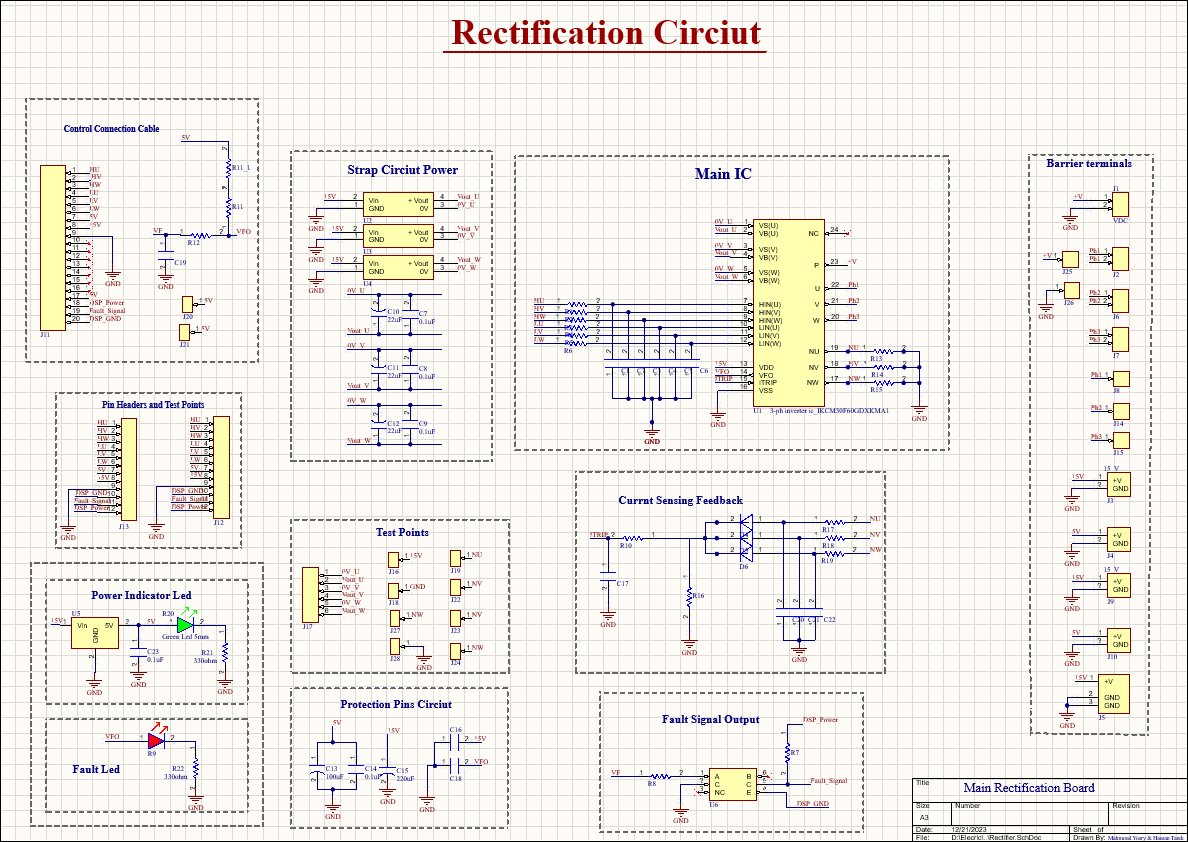
\includegraphics[width = 17cm]{image30.png}
  \caption{The Schematic of the Inverter Module}
  \label{fig:image30}
\end{figure}
We bias the bootstrap with 15V using DC/DC transformer to make an isolation. Build the protection circuit from overcurrent and overheating. The Module can shutdown itself with the ITRIP pin that has a thermistor and send a signal (Volt Fault Out) to the microcontroller to alarm the fault.
%%%%%%%%%%%%%%%%%%%%%%%%%%%%%%%%%%%%%%%%%%%%%%%%%%%%%%%%%%%%%%%%%%%%%%%%%%%%%%%%%%%%%%%%%%%%

%%%%%%%%%%%%%%%%%%%%%%%%%%%%%%%%%%%%%%%%%%%%%%%%%%%%%%%%%%%%%%%%%%%%%%%%%%%%%%%%%%%%%%%%%%%%
\subsubsection{The PCB 3D Model}
\begin{figure}[h!]
  \centering
  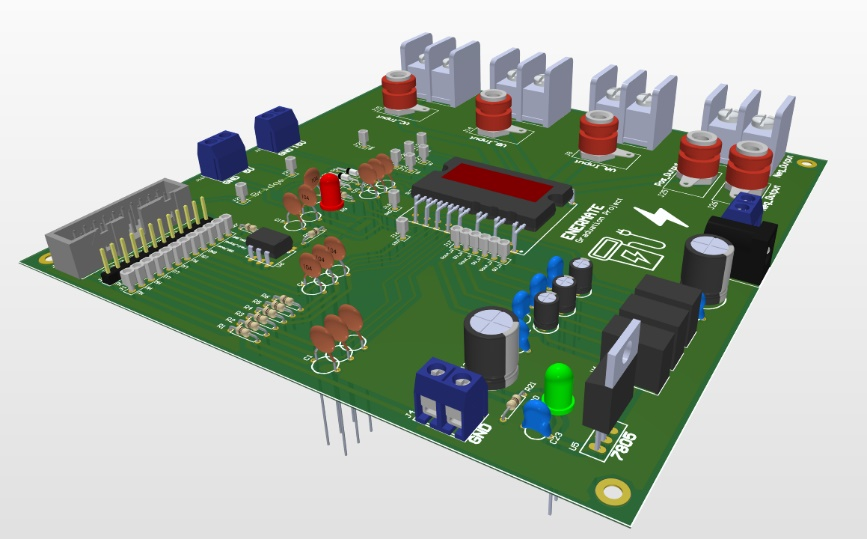
\includegraphics[width = 12cm]{image31.png}
  \caption{The PCB 3D Model of the Inverter Circuit}
  \label{fig:image31}
\end{figure}
%%%%%%%%%%%%%%%%%%%%%%%%%%%%%%%%%%%%%%%%%%%%%%%%%%%%%%%%%%%%%%%%%%%%%%%%%%%%%%%%%%%%%%%%%%%%

%%%%%%%%%%%%%%%%%%%%%%%%%%%%%%%%%%%%%%%%%%%%%%%%%%%%%%%%%%%%%%%%%%%%%%%%%%%%%%%%%%%%%%%%%%%%
\subsection{The Current Sensor}
The core of our topology is the closed loop feedback, so the measurement must be as we could to be accurate. We have chosen CAS transducer, the latest version of the LTS series. The nominal current is 25A to help us with future product.

The transducer has a multifunctional primary circuit that changes the nominal current lower to get more accuracy.
\begin{table}[h!]
  \centering
  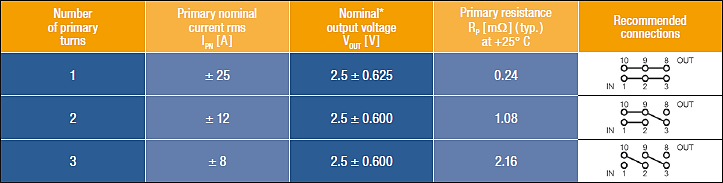
\includegraphics[width=14cm]{table2.png}
  \caption{Recommended Connections for Different Sensitivities}
\end{table}
\begin{figure}[h!]
  \centering
  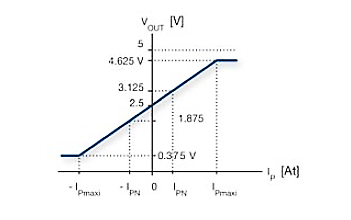
\includegraphics[width = 12cm]{image32.png}
  \caption{$V_{out}$ VS $I_{p}$ Plot}
  \label{fig:image32}
\end{figure}
In our Prototype we used the second technique that nominal current 12A.The most advantage is that the output signal does not need to rescale or biasing and ready to send to the microcontroller.
%%%%%%%%%%%%%%%%%%%%%%%%%%%%%%%%%%%%%%%%%%%%%%%%%%%%%%%%%%%%%%%%%%%%%%%%%%%%%%%%%%%%%%%%%%%%

%%%%%%%%%%%%%%%%%%%%%%%%%%%%%%%%%%%%%%%%%%%%%%%%%%%%%%%%%%%%%%%%%%%%%%%%%%%%%%%%%%%%%%%%%%%%
\subsubsection{The Hardware Schematic}
\begin{figure}[h!]
  \centering
  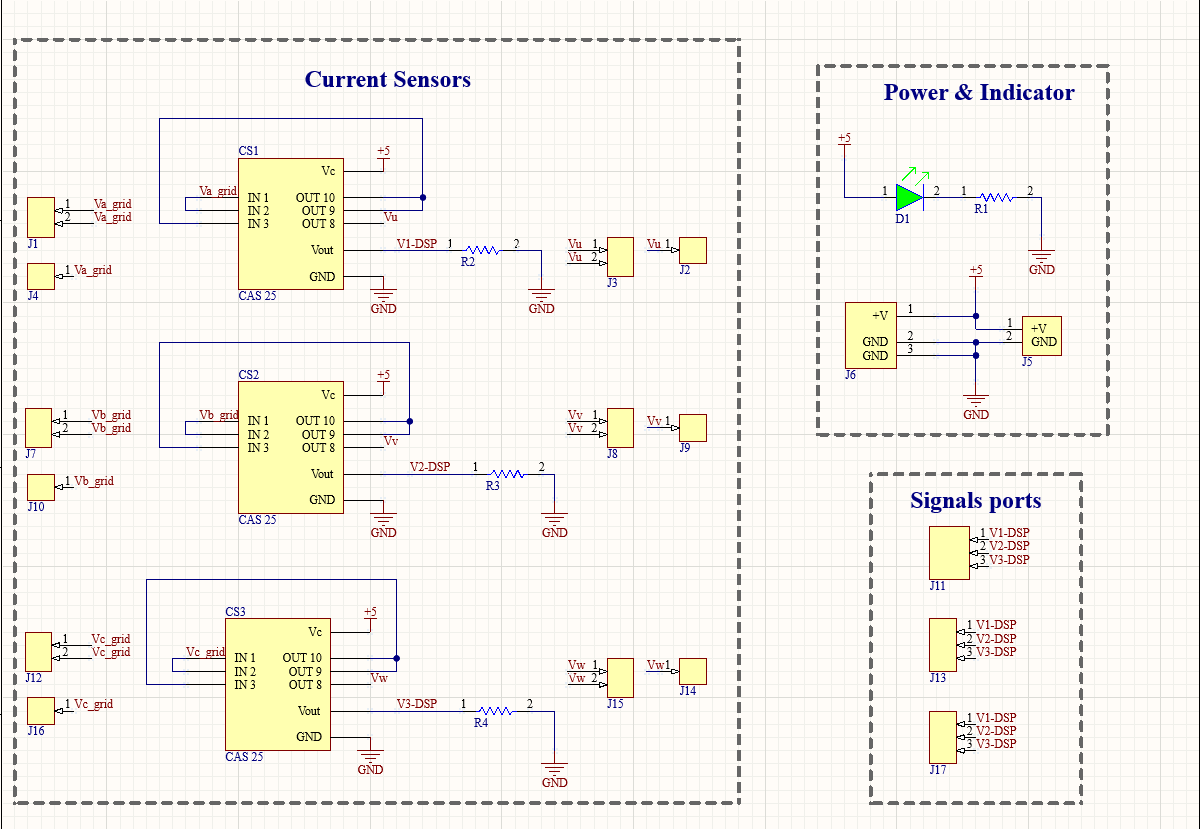
\includegraphics[width = 17cm]{image33.png}
  \caption{The Schematic of the Current Sensor}
  \label{fig:image33}
\end{figure}
%%%%%%%%%%%%%%%%%%%%%%%%%%%%%%%%%%%%%%%%%%%%%%%%%%%%%%%%%%%%%%%%%%%%%%%%%%%%%%%%%%%%%%%%%%%%

%%%%%%%%%%%%%%%%%%%%%%%%%%%%%%%%%%%%%%%%%%%%%%%%%%%%%%%%%%%%%%%%%%%%%%%%%%%%%%%%%%%%%%%%%%%%
\subsubsection{The PCB 3D Model}
\begin{figure}[h!]
  \centering
  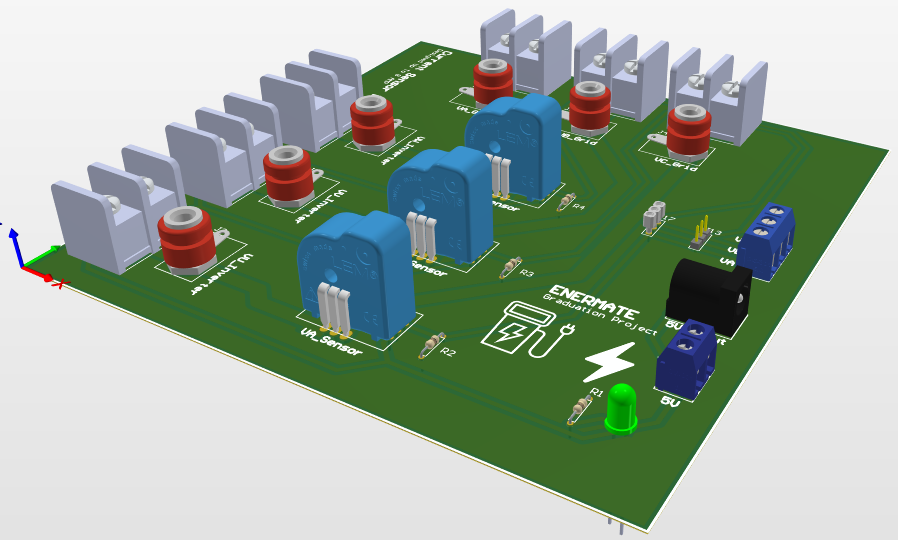
\includegraphics[width = 12cm]{image34.png}
  \caption{The PCB 3D Model of the Current Sensor}
  \label{fig:image34}
\end{figure}
%%%%%%%%%%%%%%%%%%%%%%%%%%%%%%%%%%%%%%%%%%%%%%%%%%%%%%%%%%%%%%%%%%%%%%%%%%%%%%%%%%%%%%%%%%%%

%%%%%%%%%%%%%%%%%%%%%%%%%%%%%%%%%%%%%%%%%%%%%%%%%%%%%%%%%%%%%%%%%%%%%%%%%%%%%%%%%%%%%%%%%%%%
\subsection{The Voltage Sensor}
We have chosen LV 25-P voltage transducer to get the voltage feedback
%%%%%%%%%%%%%%%%%%%%%%%%%%%%%%%%%%%%%%%%%%%%%%%%%%%%%%%%%%%%%%%%%%%%%%%%%%%%%%%%%%%%%%%%%%%%

%%%%%%%%%%%%%%%%%%%%%%%%%%%%%%%%%%%%%%%%%%%%%%%%%%%%%%%%%%%%%%%%%%%%%%%%%%%%%%%%%%%%%%%%%%%%
\subsubsection{The Features}
\begin{itemize}
  \item Current equal to 10mA and Voltage ranging from 10v up to 500v
  \item Excellent accuracy
  \item	Incredibly good linearity
  \item	Low thermal drift
  \item	Low response time
  \item	High bandwidth
  \item	High immunity to external interference
  \item	Low disturbance in common mode.
\end{itemize}
This transducer needs an external circuit to rescale and biasing the output signal before the controller, so we used an Op-Amp circuit after simulating it and get the desired output.

The transducer and the op-amp needed a positive and negative source power, so we used this topology to get the negative source.
\begin{figure}[h!]
  \centering
  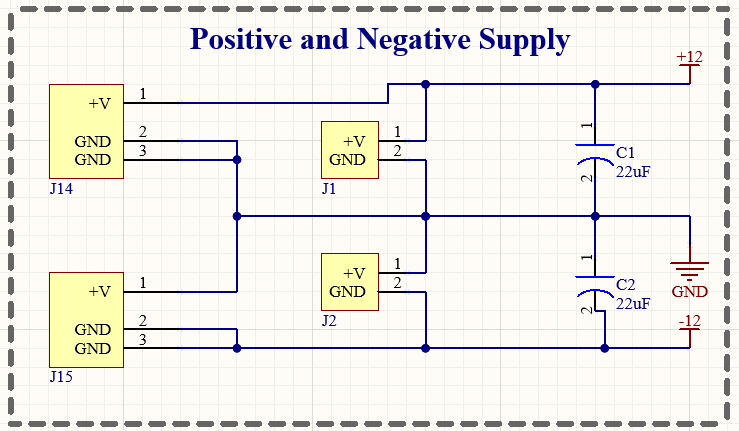
\includegraphics[width = 12cm]{image38.png}
  \caption{The Schematic of the Supply for the Voltage Sensor}
  \label{fig:image38}
\end{figure}

The following figure shows the internal connection of the sensor:
\begin{figure}[h!]
  \centering
  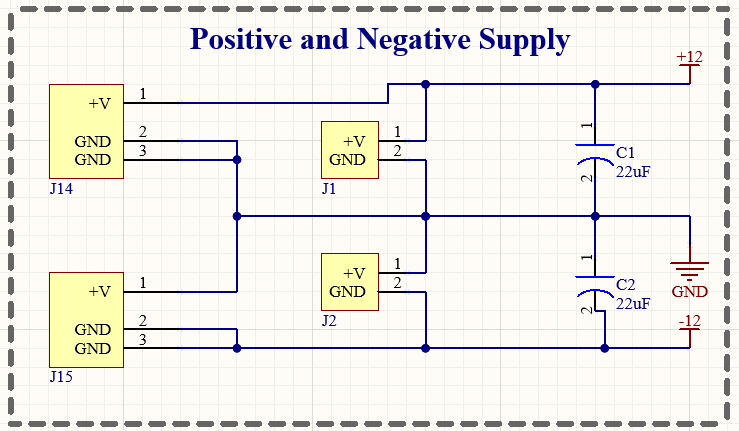
\includegraphics[width = 12cm]{image35.png}
  \caption{The Internal Connection of the Voltage Sensor}
  \label{fig:image35}
\end{figure}

Primary Side (High Voltage):
\begin{itemize}
  \item P1 and P2:  terminals Connected to the voltage to be measured.
  \item R1 (External Resistor): Sets the primary voltage range corresponding to primary current of 10 mA.
\end{itemize}
Secondary Side (Low Voltage):
\begin{itemize}
  \item +Vc: Connect this terminal to a positive power supply (5 to 15 V DC).
  \item -Vc: Connect this terminal to the negative power supply.
  \item	OUT: signal to the microcontroller
  \item	Rm (Scaling Resistor): Sets the output voltage range and sensitivity.
\end{itemize}
The resistors values can be calculated using the following equations:
\begin{equation}
  R_{m} = \ \frac{V_{out}}{I_{out}} = 132\Omega
  \label{equation:eq44}
\end{equation}
where
\begin{itemize}
  \item \(V_{out}\) is the desired output voltage. (designed for 3.3v)
  \item \(I_{out}\) is the secondary circuit current.
\end{itemize}
\begin{equation}
  R_{1} = \ \frac{V_{in}}{I_{p}} = 50K\Omega
  \label{equation:eq45}
\end{equation}
where \(V_{in}\) is equal to 500v and \(I_{out}\) is 10mA.
%%%%%%%%%%%%%%%%%%%%%%%%%%%%%%%%%%%%%%%%%%%%%%%%%%%%%%%%%%%%%%%%%%%%%%%%%%%%%%%%%%%%%%%%%%%%

%%%%%%%%%%%%%%%%%%%%%%%%%%%%%%%%%%%%%%%%%%%%%%%%%%%%%%%%%%%%%%%%%%%%%%%%%%%%%%%%%%%%%%%%%%%%
\subsubsection{Interfacing with Microcontroller - Op-Amp Technique}
In case of AC voltage measurements, dsp cannot receives negative voltage So we need to shift the signal out of the transducer to the positive and rescale it to get the desired output. Opamp adder circuit will preform this operation to convert .(-3.3v,3.3v) to (0v,3.3v).

\emph{Procedures to Design the Op-Amp circuit}
\begin{figure}[h!]
  \centering
  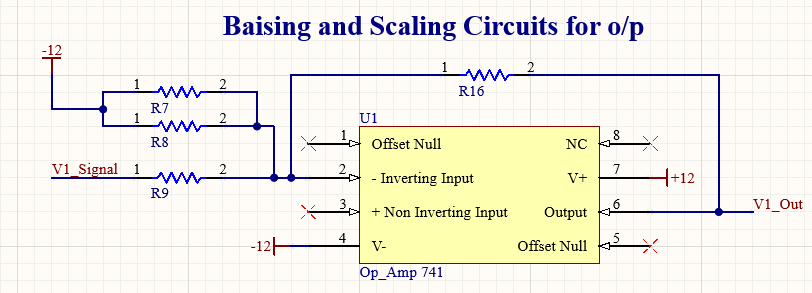
\includegraphics[width = 12cm]{image36.png}
  \caption{Op-Amp Circuit}
  \label{fig:image36}
\end{figure}
where the first terminal represents the scale of input signal and the second terminal is the shift for scaled signal.

For input signal from sensor ,the AC voltage is first scaled to half, then shifted above x axis by this scaled value to obtain its peak positive value (\(V_{in}\)) and 0v.
\begin{equation}
  -V_{out}=\left(\frac{R_{f}}{R_{1}}\ast V_{in}\right)+\left(\frac{R_{f}}{R_{2}}\ast V2\right)
  \label{equation:eq46}
\end{equation}
for AC \(V_{in}\) = 3.3V
\begin{figure}[h!]
  \centering
  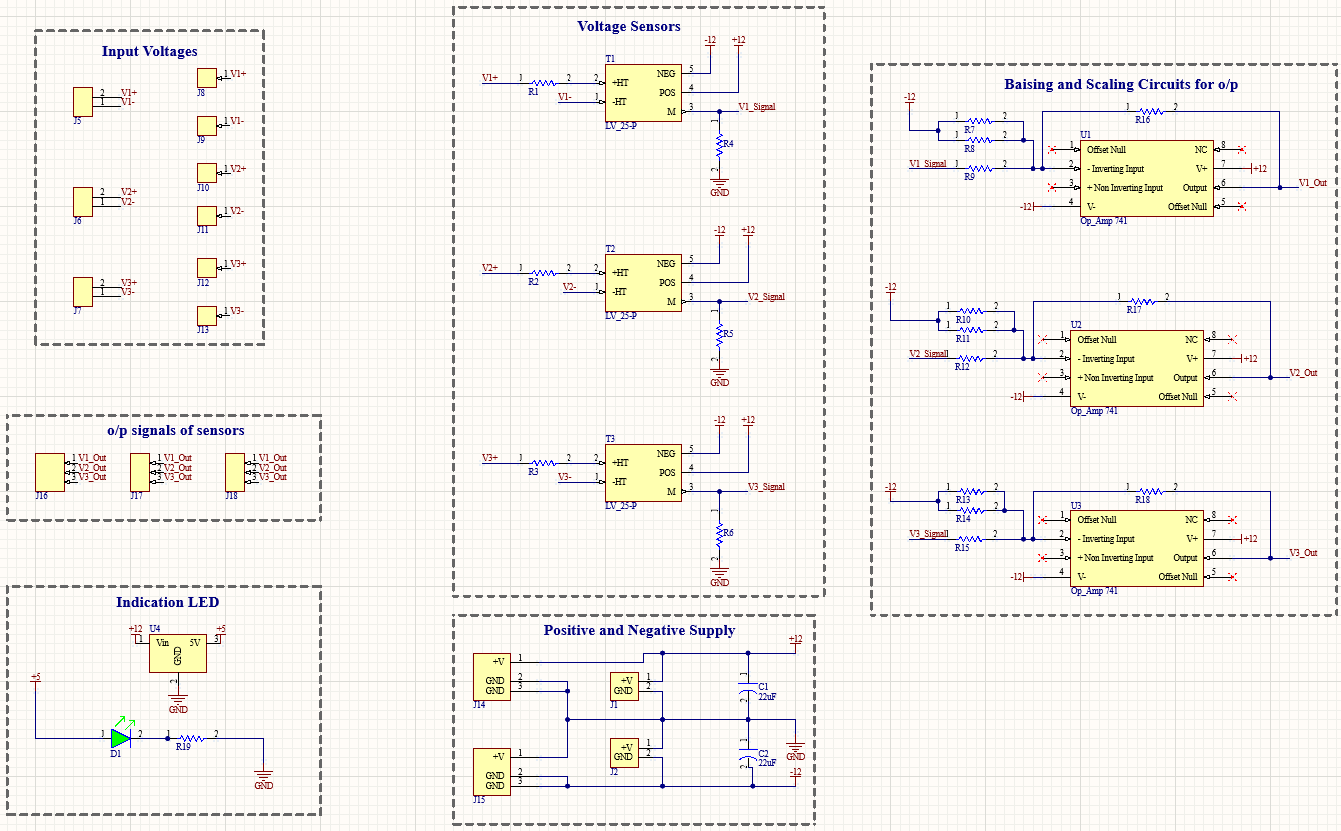
\includegraphics[width = 15cm]{image37.png}
  \caption{The Circuit Diagram of the Op-Amp}
  \label{fig:image37}
\end{figure}
\begin{enumerate}
  \item Scale the input signal to \(\frac{1}{2}V_{in}\)
  \newline\(\frac{R_{f}}{R1}\ast V_{in}=3.3/2,   assume R_{f} =10k\Omega , so R_{1} =20k\Omega\)
  \item Shift by \(\frac{1}{2}V_{in}\)
  \newline\(\frac{R_{f}}{R_{2}}\ast(V_{2})=3.3/2  ,assume V_{2} =-12v , so R_{2} = 72.7k\Omega\)
\end{enumerate}
\begin{figure}[h!]
  \centering
  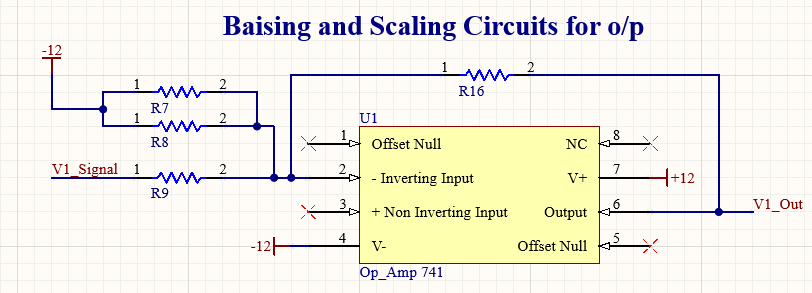
\includegraphics[width = 16cm]{image39.png}
  \caption{The Schematic of the Op-Amp Circuit}
  \label{fig:image39}
\end{figure}
%%%%%%%%%%%%%%%%%%%%%%%%%%%%%%%%%%%%%%%%%%%%%%%%%%%%%%%%%%%%%%%%%%%%%%%%%%%%%%%%%%%%%%%%%%%%

%%%%%%%%%%%%%%%%%%%%%%%%%%%%%%%%%%%%%%%%%%%%%%%%%%%%%%%%%%%%%%%%%%%%%%%%%%%%%%%%%%%%%%%%%%%%
\subsubsection{The Hardware Schematic}
\begin{figure}[h!]
  \centering
  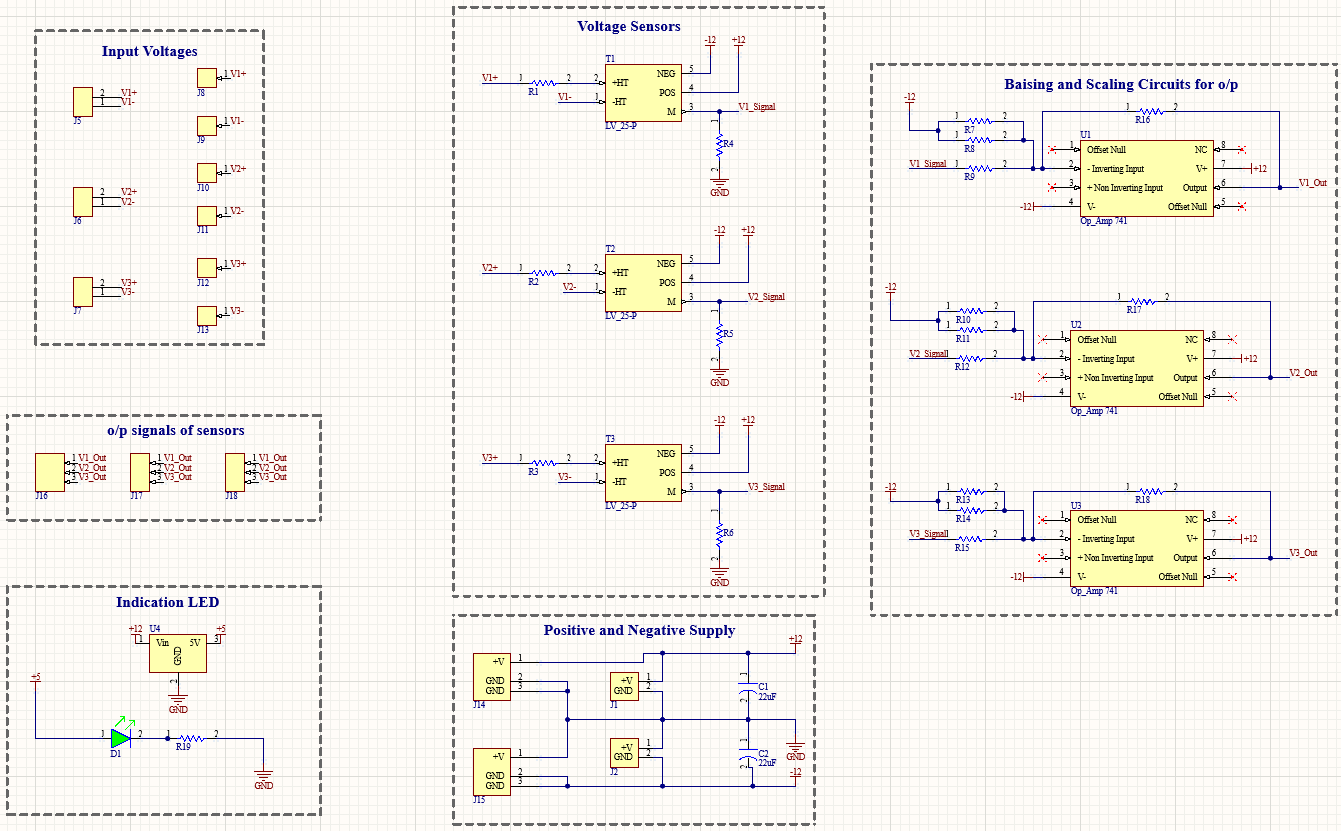
\includegraphics[width = 17cm]{image40.png}
  \caption{The Schematic of the Voltage Sensor}
  \label{fig:image40}
\end{figure}
%%%%%%%%%%%%%%%%%%%%%%%%%%%%%%%%%%%%%%%%%%%%%%%%%%%%%%%%%%%%%%%%%%%%%%%%%%%%%%%%%%%%%%%%%%%%

%%%%%%%%%%%%%%%%%%%%%%%%%%%%%%%%%%%%%%%%%%%%%%%%%%%%%%%%%%%%%%%%%%%%%%%%%%%%%%%%%%%%%%%%%%%%
\subsubsection{The PCB 3D Model}
\begin{figure}[h!]
  \centering
  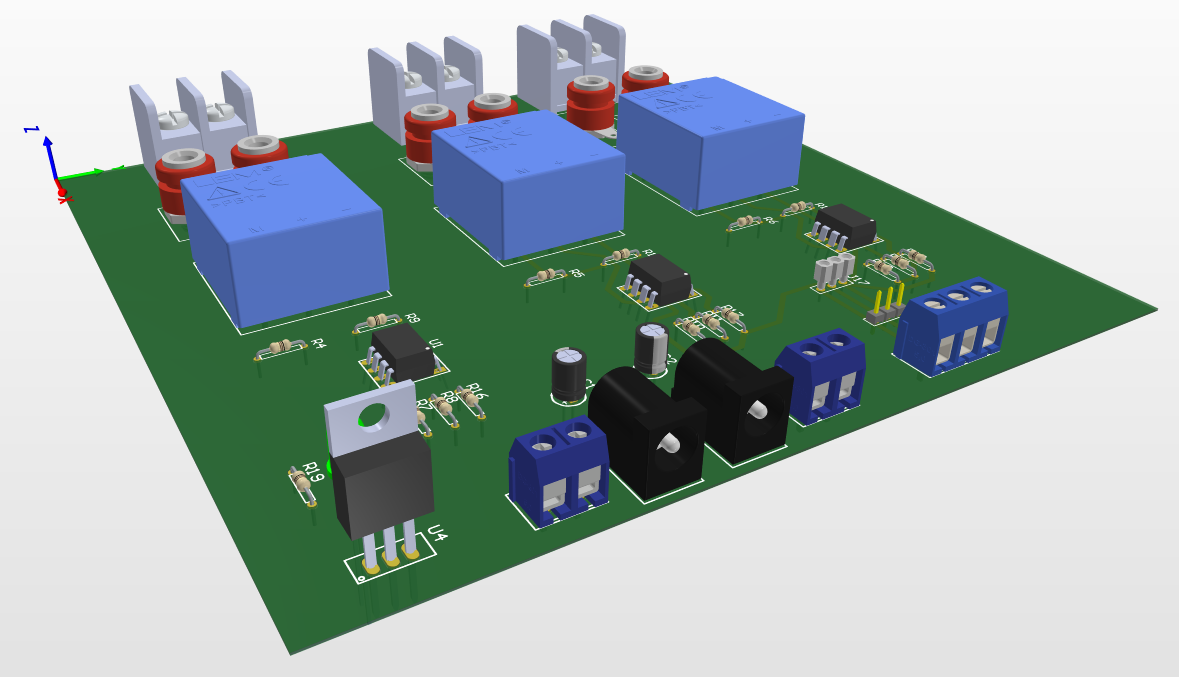
\includegraphics[width = 15cm]{image41.png}
  \caption{The PCB 3D Model of the Voltage Sensor}
  \label{fig:image41}
\end{figure}
%%%%%%%%%%%%%%%%%%%%%%%%%%%%%%%%%%%%%%%%%%%%%%%%%%%%%%%%%%%%%%%%%%%%%%%%%%%%%%%%%%%%%%%%%%%%

%%%%%%%%%%%%%%%%%%%%%%%%%%%%%%%%%%%%%%%%%%%%%%%%%%%%%%%%%%%%%%%%%%%%%%%%%%%%%%%%%%%%%%%%%%%%
\subsection{The Microcontroller}
We have chosen to use DSP LaunchpadF28069M, because it is the easier controller to generate our model on it. We built a DSP interfacing with the inverter using optocoupler circuit to make the suitable isolation.
%%%%%%%%%%%%%%%%%%%%%%%%%%%%%%%%%%%%%%%%%%%%%%%%%%%%%%%%%%%%%%%%%%%%%%%%%%%%%%%%%%%%%%%%%%%%

%%%%%%%%%%%%%%%%%%%%%%%%%%%%%%%%%%%%%%%%%%%%%%%%%%%%%%%%%%%%%%%%%%%%%%%%%%%%%%%%%%%%%%%%%%%%
\subsubsection{The Hardware Schematic}
\begin{figure}[h!]
  \centering
  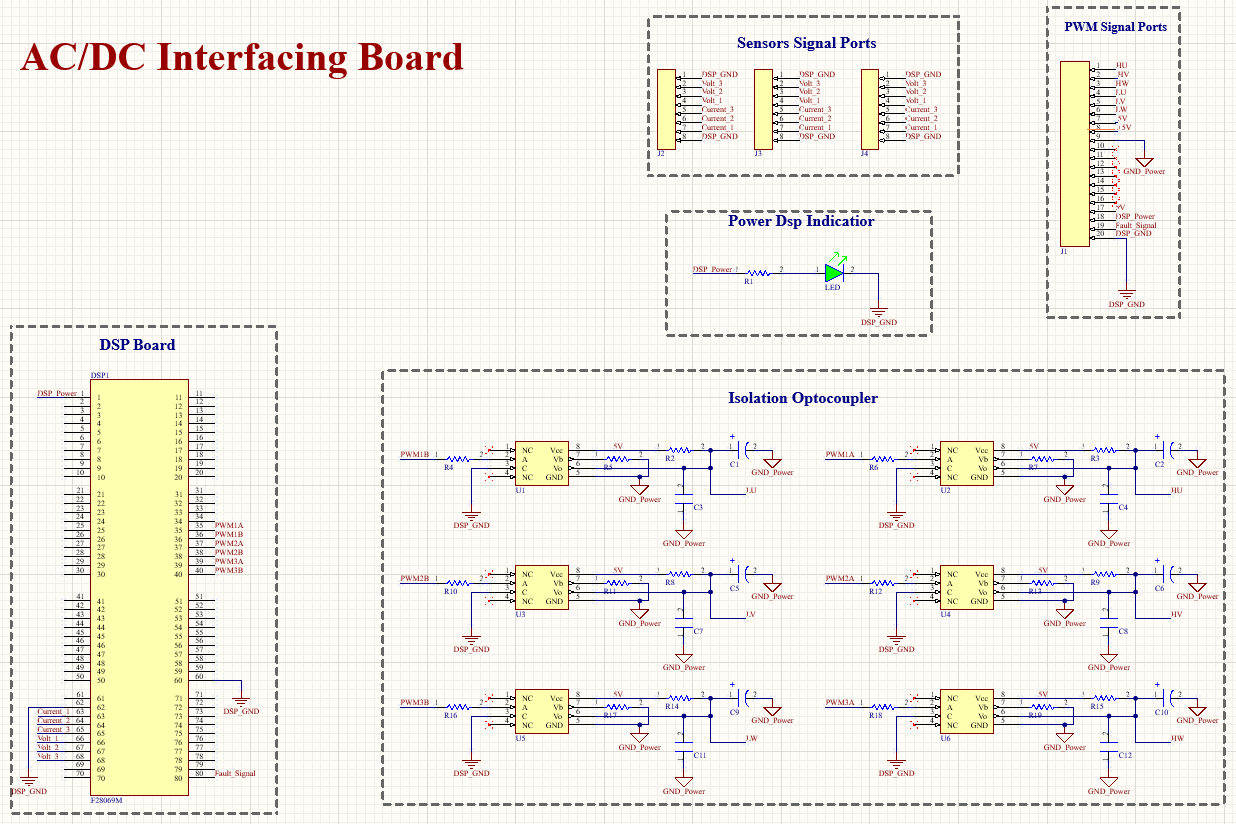
\includegraphics[width = 17cm]{image42.png}
  \caption{The Schematic of the DSP Interfacing Board}
  \label{fig:image42}
\end{figure}
%%%%%%%%%%%%%%%%%%%%%%%%%%%%%%%%%%%%%%%%%%%%%%%%%%%%%%%%%%%%%%%%%%%%%%%%%%%%%%%%%%%%%%%%%%%%

%%%%%%%%%%%%%%%%%%%%%%%%%%%%%%%%%%%%%%%%%%%%%%%%%%%%%%%%%%%%%%%%%%%%%%%%%%%%%%%%%%%%%%%%%%%%
\subsubsection{The PCB 3D Model}
\begin{figure}[h!]
  \centering
  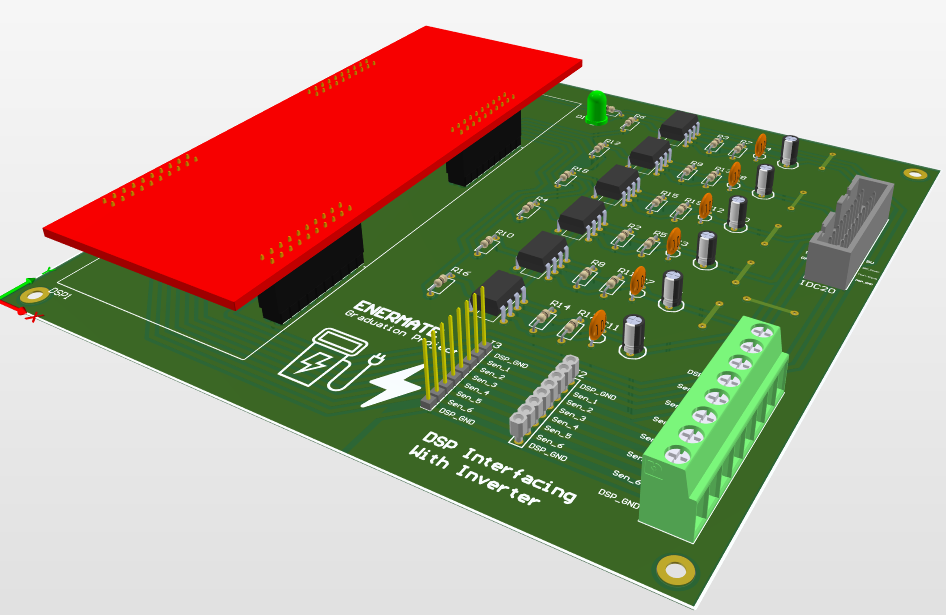
\includegraphics[width = 15cm]{image43.png}
  \caption{The PCB 3D Model of the DSP Interfacing Board}
  \label{fig:image43}
\end{figure}
%%%%%%%%%%%%%%%%%%%%%%%%%%%%%%%%%%%%%%%%%%%%%%%%%%%%%%%%%%%%%%%%%%%%%%%%%%%%%%%%%%%%%%%%%%%%

%%%%%%%%%%%%%%%%%%%%%%%%%%%%%%%%%%%%%%%%%%%%%%%%%%%%%%%%%%%%%%%%%%%%%%%%%%%%%%%%%%%%%%%%%%%%
\subsection{DC-Link}
According to our calculations that we have done in previous sections, we have designed a DC-Link to suit our project to literally link between the AC/DC Converion and the DC/DC Conversion boards.
%%%%%%%%%%%%%%%%%%%%%%%%%%%%%%%%%%%%%%%%%%%%%%%%%%%%%%%%%%%%%%%%%%%%%%%%%%%%%%%%%%%%%%%%%%%%

%%%%%%%%%%%%%%%%%%%%%%%%%%%%%%%%%%%%%%%%%%%%%%%%%%%%%%%%%%%%%%%%%%%%%%%%%%%%%%%%%%%%%%%%%%%%
\subsubsection{The Hardware Schematic}
\begin{figure}[h!]
  \centering
  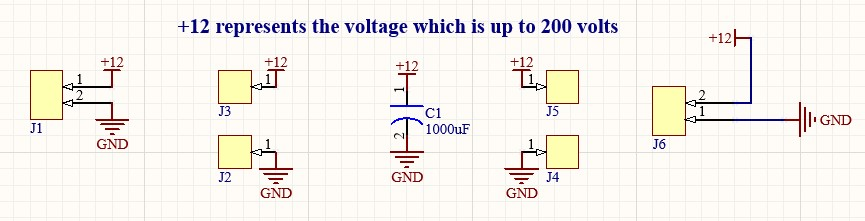
\includegraphics[width = 17cm]{image44.png}
  \caption{The Schematic of the DC-Link}
  \label{fig:image44}
\end{figure}
%%%%%%%%%%%%%%%%%%%%%%%%%%%%%%%%%%%%%%%%%%%%%%%%%%%%%%%%%%%%%%%%%%%%%%%%%%%%%%%%%%%%%%%%%%%%

%%%%%%%%%%%%%%%%%%%%%%%%%%%%%%%%%%%%%%%%%%%%%%%%%%%%%%%%%%%%%%%%%%%%%%%%%%%%%%%%%%%%%%%%%%%%
\subsubsection{The PCB 3D Model}
\begin{figure}[h!]
  \centering
  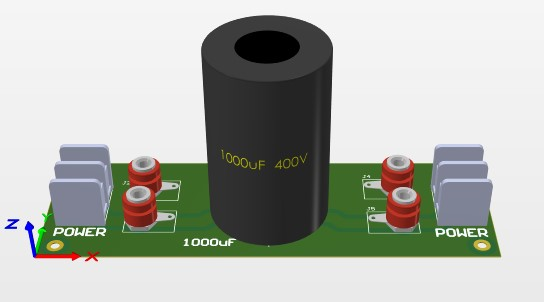
\includegraphics[width = 15cm]{image45.png}
  \caption{The PCB 3D Model of the DC-Link}
  \label{fig:image45}
\end{figure}
%%%%%%%%%%%%%%%%%%%%%%%%%%%%%%%%%%%%%%%%%%%%%%%%%%%%%%%%%%%%%%%%%%%%%%%%%%%%%%%%%%%%%%%%%%%%

\bibliographystyle{plain}
\bibliography{references}

\end{document}